% Options for packages loaded elsewhere
\PassOptionsToPackage{unicode}{hyperref}
\PassOptionsToPackage{hyphens}{url}
\PassOptionsToPackage{dvipsnames,svgnames,x11names}{xcolor}
%
\documentclass[
  letterpaper,
  DIV=11,
  numbers=noendperiod]{scrreprt}

\usepackage{amsmath,amssymb}
\usepackage{lmodern}
\usepackage{iftex}
\ifPDFTeX
  \usepackage[T1]{fontenc}
  \usepackage[utf8]{inputenc}
  \usepackage{textcomp} % provide euro and other symbols
\else % if luatex or xetex
  \usepackage{unicode-math}
  \defaultfontfeatures{Scale=MatchLowercase}
  \defaultfontfeatures[\rmfamily]{Ligatures=TeX,Scale=1}
\fi
% Use upquote if available, for straight quotes in verbatim environments
\IfFileExists{upquote.sty}{\usepackage{upquote}}{}
\IfFileExists{microtype.sty}{% use microtype if available
  \usepackage[]{microtype}
  \UseMicrotypeSet[protrusion]{basicmath} % disable protrusion for tt fonts
}{}
\makeatletter
\@ifundefined{KOMAClassName}{% if non-KOMA class
  \IfFileExists{parskip.sty}{%
    \usepackage{parskip}
  }{% else
    \setlength{\parindent}{0pt}
    \setlength{\parskip}{6pt plus 2pt minus 1pt}}
}{% if KOMA class
  \KOMAoptions{parskip=half}}
\makeatother
\usepackage{xcolor}
\setlength{\emergencystretch}{3em} % prevent overfull lines
\setcounter{secnumdepth}{5}
% Make \paragraph and \subparagraph free-standing
\ifx\paragraph\undefined\else
  \let\oldparagraph\paragraph
  \renewcommand{\paragraph}[1]{\oldparagraph{#1}\mbox{}}
\fi
\ifx\subparagraph\undefined\else
  \let\oldsubparagraph\subparagraph
  \renewcommand{\subparagraph}[1]{\oldsubparagraph{#1}\mbox{}}
\fi

\usepackage{color}
\usepackage{fancyvrb}
\newcommand{\VerbBar}{|}
\newcommand{\VERB}{\Verb[commandchars=\\\{\}]}
\DefineVerbatimEnvironment{Highlighting}{Verbatim}{commandchars=\\\{\}}
% Add ',fontsize=\small' for more characters per line
\usepackage{framed}
\definecolor{shadecolor}{RGB}{241,243,245}
\newenvironment{Shaded}{\begin{snugshade}}{\end{snugshade}}
\newcommand{\AlertTok}[1]{\textcolor[rgb]{0.68,0.00,0.00}{#1}}
\newcommand{\AnnotationTok}[1]{\textcolor[rgb]{0.37,0.37,0.37}{#1}}
\newcommand{\AttributeTok}[1]{\textcolor[rgb]{0.40,0.45,0.13}{#1}}
\newcommand{\BaseNTok}[1]{\textcolor[rgb]{0.68,0.00,0.00}{#1}}
\newcommand{\BuiltInTok}[1]{\textcolor[rgb]{0.00,0.23,0.31}{#1}}
\newcommand{\CharTok}[1]{\textcolor[rgb]{0.13,0.47,0.30}{#1}}
\newcommand{\CommentTok}[1]{\textcolor[rgb]{0.37,0.37,0.37}{#1}}
\newcommand{\CommentVarTok}[1]{\textcolor[rgb]{0.37,0.37,0.37}{\textit{#1}}}
\newcommand{\ConstantTok}[1]{\textcolor[rgb]{0.56,0.35,0.01}{#1}}
\newcommand{\ControlFlowTok}[1]{\textcolor[rgb]{0.00,0.23,0.31}{#1}}
\newcommand{\DataTypeTok}[1]{\textcolor[rgb]{0.68,0.00,0.00}{#1}}
\newcommand{\DecValTok}[1]{\textcolor[rgb]{0.68,0.00,0.00}{#1}}
\newcommand{\DocumentationTok}[1]{\textcolor[rgb]{0.37,0.37,0.37}{\textit{#1}}}
\newcommand{\ErrorTok}[1]{\textcolor[rgb]{0.68,0.00,0.00}{#1}}
\newcommand{\ExtensionTok}[1]{\textcolor[rgb]{0.00,0.23,0.31}{#1}}
\newcommand{\FloatTok}[1]{\textcolor[rgb]{0.68,0.00,0.00}{#1}}
\newcommand{\FunctionTok}[1]{\textcolor[rgb]{0.28,0.35,0.67}{#1}}
\newcommand{\ImportTok}[1]{\textcolor[rgb]{0.00,0.46,0.62}{#1}}
\newcommand{\InformationTok}[1]{\textcolor[rgb]{0.37,0.37,0.37}{#1}}
\newcommand{\KeywordTok}[1]{\textcolor[rgb]{0.00,0.23,0.31}{#1}}
\newcommand{\NormalTok}[1]{\textcolor[rgb]{0.00,0.23,0.31}{#1}}
\newcommand{\OperatorTok}[1]{\textcolor[rgb]{0.37,0.37,0.37}{#1}}
\newcommand{\OtherTok}[1]{\textcolor[rgb]{0.00,0.23,0.31}{#1}}
\newcommand{\PreprocessorTok}[1]{\textcolor[rgb]{0.68,0.00,0.00}{#1}}
\newcommand{\RegionMarkerTok}[1]{\textcolor[rgb]{0.00,0.23,0.31}{#1}}
\newcommand{\SpecialCharTok}[1]{\textcolor[rgb]{0.37,0.37,0.37}{#1}}
\newcommand{\SpecialStringTok}[1]{\textcolor[rgb]{0.13,0.47,0.30}{#1}}
\newcommand{\StringTok}[1]{\textcolor[rgb]{0.13,0.47,0.30}{#1}}
\newcommand{\VariableTok}[1]{\textcolor[rgb]{0.07,0.07,0.07}{#1}}
\newcommand{\VerbatimStringTok}[1]{\textcolor[rgb]{0.13,0.47,0.30}{#1}}
\newcommand{\WarningTok}[1]{\textcolor[rgb]{0.37,0.37,0.37}{\textit{#1}}}

\providecommand{\tightlist}{%
  \setlength{\itemsep}{0pt}\setlength{\parskip}{0pt}}\usepackage{longtable,booktabs,array}
\usepackage{calc} % for calculating minipage widths
% Correct order of tables after \paragraph or \subparagraph
\usepackage{etoolbox}
\makeatletter
\patchcmd\longtable{\par}{\if@noskipsec\mbox{}\fi\par}{}{}
\makeatother
% Allow footnotes in longtable head/foot
\IfFileExists{footnotehyper.sty}{\usepackage{footnotehyper}}{\usepackage{footnote}}
\makesavenoteenv{longtable}
\usepackage{graphicx}
\makeatletter
\def\maxwidth{\ifdim\Gin@nat@width>\linewidth\linewidth\else\Gin@nat@width\fi}
\def\maxheight{\ifdim\Gin@nat@height>\textheight\textheight\else\Gin@nat@height\fi}
\makeatother
% Scale images if necessary, so that they will not overflow the page
% margins by default, and it is still possible to overwrite the defaults
% using explicit options in \includegraphics[width, height, ...]{}
\setkeys{Gin}{width=\maxwidth,height=\maxheight,keepaspectratio}
% Set default figure placement to htbp
\makeatletter
\def\fps@figure{htbp}
\makeatother
\newlength{\cslhangindent}
\setlength{\cslhangindent}{1.5em}
\newlength{\csllabelwidth}
\setlength{\csllabelwidth}{3em}
\newlength{\cslentryspacingunit} % times entry-spacing
\setlength{\cslentryspacingunit}{\parskip}
\newenvironment{CSLReferences}[2] % #1 hanging-ident, #2 entry spacing
 {% don't indent paragraphs
  \setlength{\parindent}{0pt}
  % turn on hanging indent if param 1 is 1
  \ifodd #1
  \let\oldpar\par
  \def\par{\hangindent=\cslhangindent\oldpar}
  \fi
  % set entry spacing
  \setlength{\parskip}{#2\cslentryspacingunit}
 }%
 {}
\usepackage{calc}
\newcommand{\CSLBlock}[1]{#1\hfill\break}
\newcommand{\CSLLeftMargin}[1]{\parbox[t]{\csllabelwidth}{#1}}
\newcommand{\CSLRightInline}[1]{\parbox[t]{\linewidth - \csllabelwidth}{#1}\break}
\newcommand{\CSLIndent}[1]{\hspace{\cslhangindent}#1}

\KOMAoption{captions}{tableheading}
\makeatletter
\makeatother
\makeatletter
\@ifpackageloaded{bookmark}{}{\usepackage{bookmark}}
\makeatother
\makeatletter
\@ifpackageloaded{caption}{}{\usepackage{caption}}
\AtBeginDocument{%
\ifdefined\contentsname
  \renewcommand*\contentsname{Table of contents}
\else
  \newcommand\contentsname{Table of contents}
\fi
\ifdefined\listfigurename
  \renewcommand*\listfigurename{List of Figures}
\else
  \newcommand\listfigurename{List of Figures}
\fi
\ifdefined\listtablename
  \renewcommand*\listtablename{List of Tables}
\else
  \newcommand\listtablename{List of Tables}
\fi
\ifdefined\figurename
  \renewcommand*\figurename{Figure}
\else
  \newcommand\figurename{Figure}
\fi
\ifdefined\tablename
  \renewcommand*\tablename{Table}
\else
  \newcommand\tablename{Table}
\fi
}
\@ifpackageloaded{float}{}{\usepackage{float}}
\floatstyle{ruled}
\@ifundefined{c@chapter}{\newfloat{codelisting}{h}{lop}}{\newfloat{codelisting}{h}{lop}[chapter]}
\floatname{codelisting}{Listing}
\newcommand*\listoflistings{\listof{codelisting}{List of Listings}}
\makeatother
\makeatletter
\@ifpackageloaded{caption}{}{\usepackage{caption}}
\@ifpackageloaded{subcaption}{}{\usepackage{subcaption}}
\makeatother
\makeatletter
\@ifpackageloaded{tcolorbox}{}{\usepackage[many]{tcolorbox}}
\makeatother
\makeatletter
\@ifundefined{shadecolor}{\definecolor{shadecolor}{rgb}{.97, .97, .97}}
\makeatother
\makeatletter
\makeatother
\ifLuaTeX
  \usepackage{selnolig}  % disable illegal ligatures
\fi
\IfFileExists{bookmark.sty}{\usepackage{bookmark}}{\usepackage{hyperref}}
\IfFileExists{xurl.sty}{\usepackage{xurl}}{} % add URL line breaks if available
\urlstyle{same} % disable monospaced font for URLs
\hypersetup{
  pdftitle={Transporte en nanoestructuras de Bi},
  pdfauthor={Montserrat Navarro Espino},
  colorlinks=true,
  linkcolor={blue},
  filecolor={Maroon},
  citecolor={Blue},
  urlcolor={Blue},
  pdfcreator={LaTeX via pandoc}}

\title{Transporte en nanoestructuras de Bi}
\author{Montserrat Navarro Espino}
\date{7/31/2023}

\begin{document}
\maketitle
\ifdefined\Shaded\renewenvironment{Shaded}{\begin{tcolorbox}[boxrule=0pt, borderline west={3pt}{0pt}{shadecolor}, breakable, interior hidden, frame hidden, enhanced, sharp corners]}{\end{tcolorbox}}\fi

\renewcommand*\contentsname{Table of contents}
{
\hypersetup{linkcolor=}
\setcounter{tocdepth}{2}
\tableofcontents
}
\bookmarksetup{startatroot}

\hypertarget{prefacio}{%
\chapter*{Prefacio}\label{prefacio}}
\addcontentsline{toc}{chapter}{Prefacio}

Este es un sitio creado con Quarto y y publicado a través de GitHub
Pages. En él se encuentran conceptos clave para el estudio del
transporte electrónico en nanoestructuras de bismuto.

La elaboración de estas notas tiene como propósito brindar acceso a los
resultados del trabajo de investigación desempeñado por la autora en el
Programa de Maestría en Ciencias Químicas.

\bookmarksetup{startatroot}

\hypertarget{introducciuxf3n}{%
\chapter{Introducción}\label{introducciuxf3n}}

El bismuto es uno de los elementos químicos más pesados y con un mayor
tiempo de vida media (\(2 \times 10 ^{19}\) años aproximadamente)
\cite{Kanatzidis2020,Marcillac2003}. Por ende, posee un enorme
acoplamiento espín-orbita (SOC, por sus siglas en inglés) y sus
electrones presentan efectos relativistas
\cite{Tatewaki2017, Bucinsky2016}. El cristal de bismuto es un semimetal
en el que se han observado diversas propiedades y fenómenos cuánticos de
interés, siendo uno de ellos la topología de su estructura electrónica
\cite{Ito2016}.

La estructura electrónica de Bi prístino ha sido considerada por un
largo tiempo como topológicamente trivial, lo cual implica que Sin
embargo, a través de varios experimentos empleando la espectroscopía de
fotoemisión con resolución angular (ARPES, por sus siglas en inglés), se
encontró que las bandas de la superficie poseen una topología no trivial
\cite{Ohtsubo2013,Perfetti2015,}, como se observa en la Fig.
\ref{fig:ArpesBi3d}.

En el año 2018, se realizó un esfuerzo excepcional en este ámbito, donde
fue identificada la naturaleza topológica de orden superior de la
estructura electrónica de bismuto \cite{Schindler2018}. En dicho trabajo
se identificaron estados de arista Figure~\ref{fig-expBihs}, o
\textit{hinge states}, los cuales están protegidos globalmente por la
simetría de reversión temporal (\(TRS\)), y discretamente por la
simetría rotacional de tercer orden (\(\hat{\mathcal{C}_3}\)) y la
simetría de inversión del cristal de bismuto (\(\hat{\mathcal{I}}\)).

\begin{figure}

{\centering 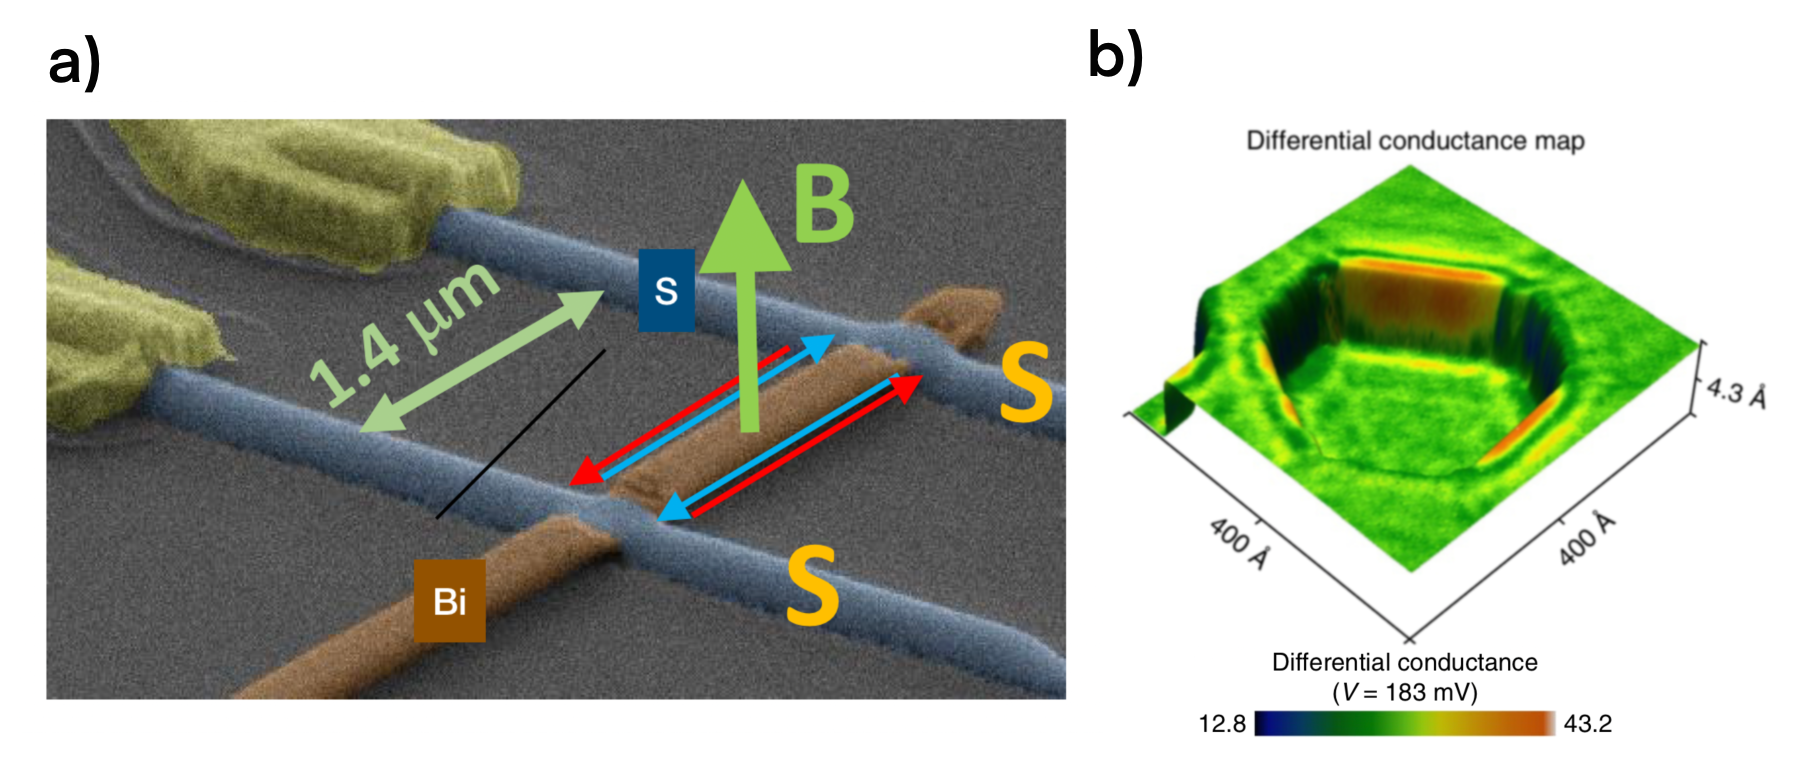
\includegraphics{./images/Exp-bitop.png}

}

\caption{\label{fig-expBihs}Detección experimental de los estados de
arista. a) Experimento STM donde se observan estados alternados y
fuertemente localizados en el borde de Bi (111). b) Junta de Josephson
S/Bi/S donde se detecta corriente fluye a través de canales
extremadamente estrechos (unidimensionales) \cite{Schindler2018}.}

\end{figure}

\bookmarksetup{startatroot}

\hypertarget{geometruxeda-de-bismuto}{%
\chapter{Geometría de bismuto}\label{geometruxeda-de-bismuto}}

\hypertarget{estructura-cristalina-de-bismuto}{%
\section{Estructura cristalina de
bismuto}\label{estructura-cristalina-de-bismuto}}

\hypertarget{espacio-real}{%
\subsection{Espacio Real}\label{espacio-real}}

El bismuto (Bi) es un elemento químico cuyo arreglo cristalino consiste
de una celda unitaria romboédrica que contiene dos átomos
\cite{Falicov1965}, cada uno de ellos con tres primeros vecinos y tres
segundos vecinos \cite{HOFMANN2006}, como se señala en la Fig.
(\textbf{RomboRealRec?}) a).

\begin{figure}

{\centering 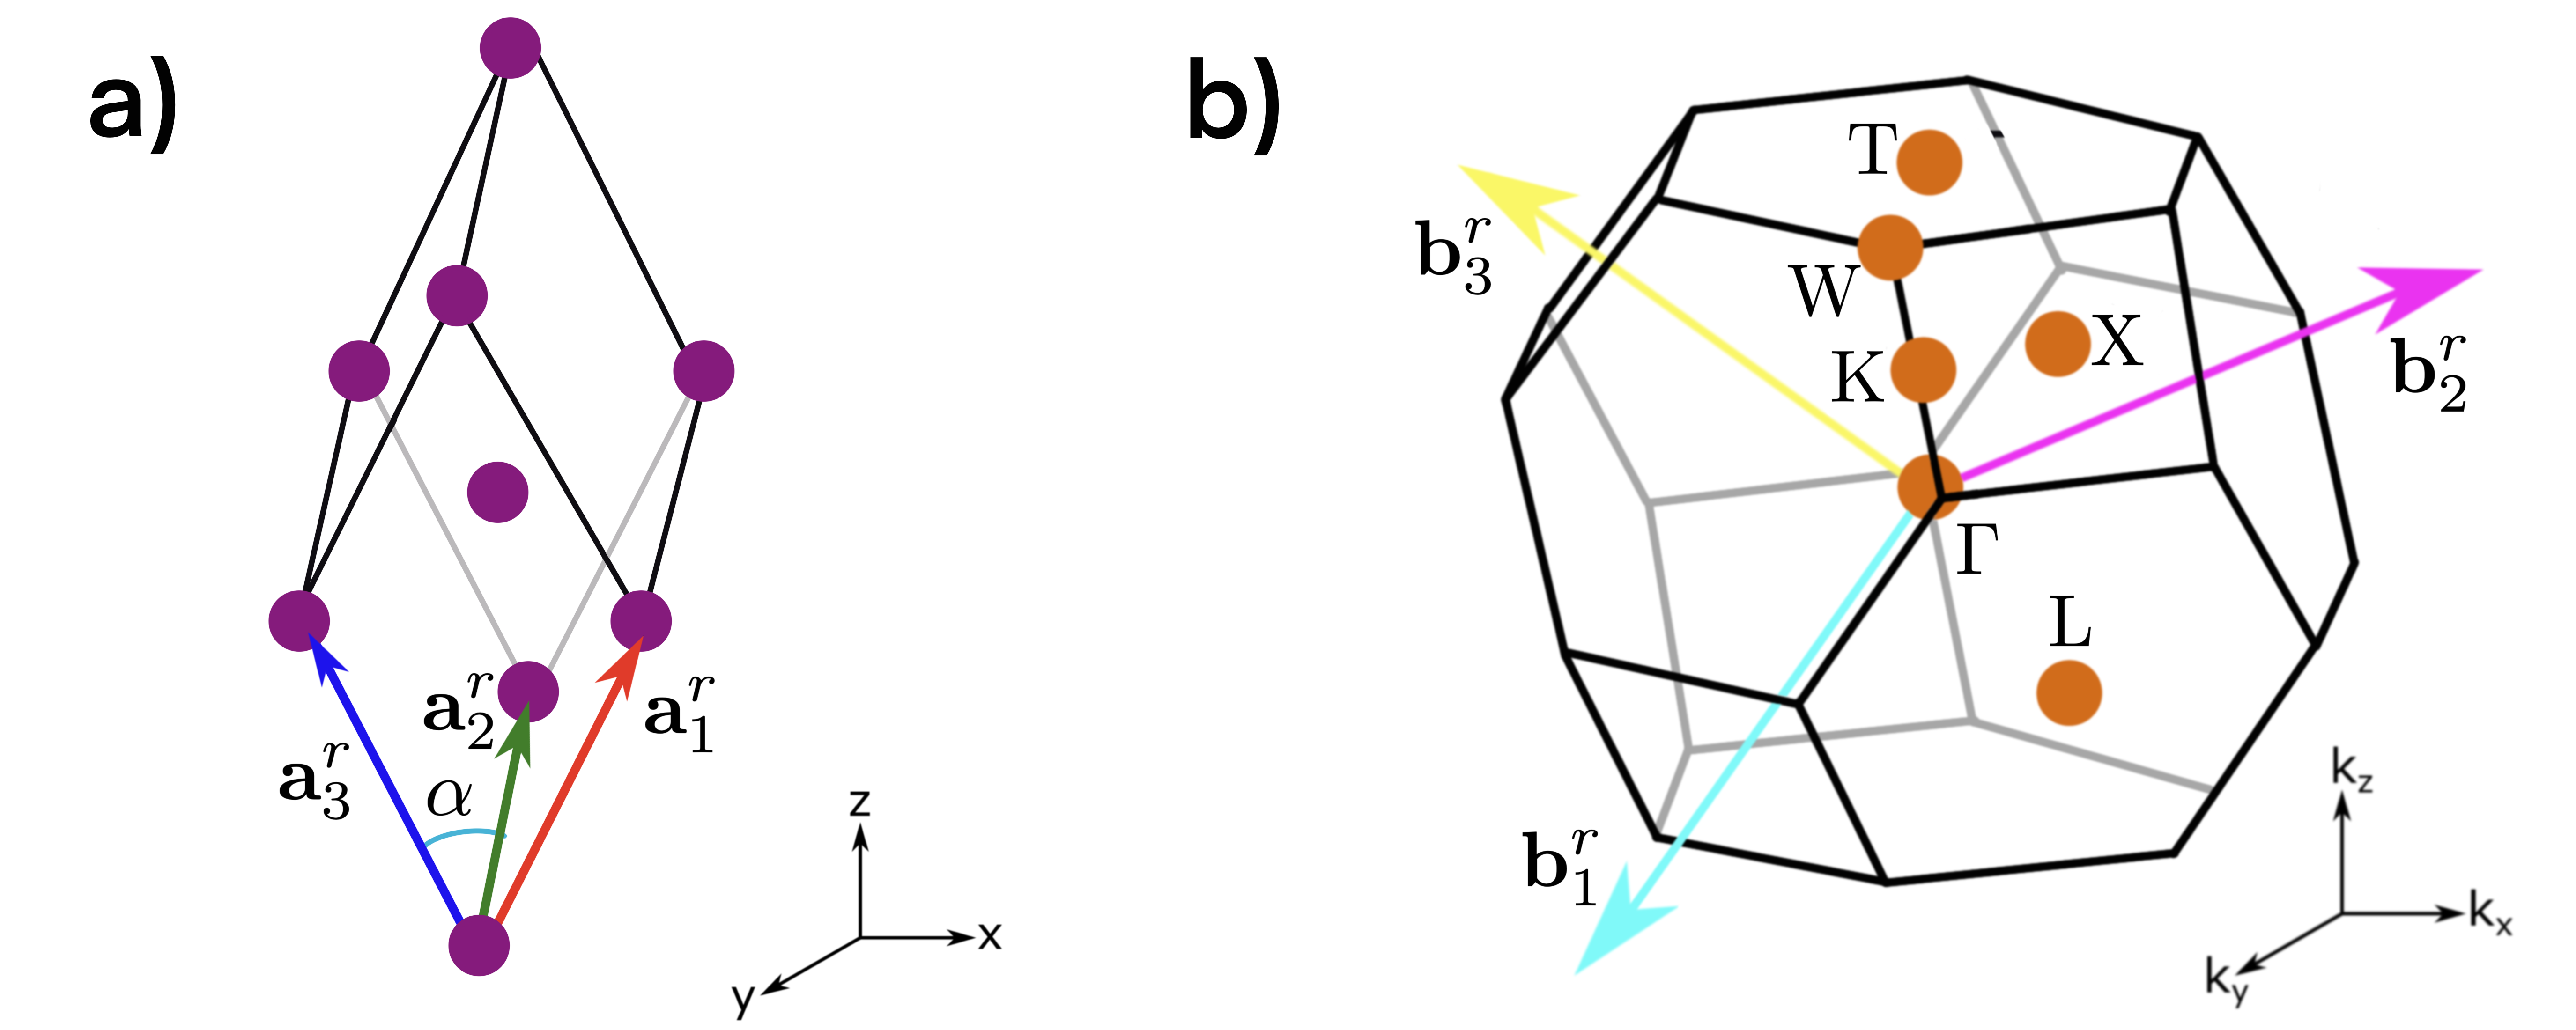
\includegraphics{./images/RombRealRec.png}

}

\caption{\label{fig-RomboRealRecBi}a) Celda romboédrica de bismuto en el
espacio real, con los vectores de red \(\mathbf{a}^r_n\) (\(n=1,2,3\)).
b) Primera zona de Brillouin de la estructura romboédrica del Bi, con
los vectores \(\mathbf{b}^r_n\) y los puntos de alta simetría
(naranja).}

\end{figure}

La estructura romboédrica de bismuto se esquematiza en la Fig.
Figure~\ref{fig-RomboRealRecBi} (a), donde los vectores de la red en el
espacio real son:

\[
    \mathbf{a}_1^r = \left ( -\frac{1}{2}a , -\frac{\sqrt{3}}{6}a , \frac{1}{3}c \right ) \hspace{10mm}
    \mathbf{a}_2^r = \left (  \frac{1}{2}a , -\frac{\sqrt{3}}{6}a , \frac{1}{3}c \right ) \hspace{10mm}
    \mathbf{a}_3^r = \left (             0 , -\frac{\sqrt{3}}{3}a , \frac{1}{3}c \right ) 
\]

siendo \(a=4.5332\) Å , \(c= 11.7967\) Å y \(\alpha = 57^{\circ}19'\)
\cite{LiuandAllen1995}.

El grupo espacial de la estructura cristalina es \(R\bar{3}m\) y su
grupo puntual es el \(D_{3d}\). Por lo tanto, las operaciones de
simetría espacial que caracterizan este arreglo cristalino son
\cite{Hsu2019}:

\begin{itemize}
\tightlist
\item
  la identidad (\(\hat{E}\)),
\item
  la inversión (\(\hat{I}\)),
\item
  las rotaciones de 120\(^{\circ}\) (\(\hat{C}_3\)) respecto el eje
  \(z\) y 180\(^{\circ}\) (\(\hat{C}_2\)) respecto el eje \(y\) y
\item
  los planos de reflexión \(\mathcal{M}_a\), \(\mathcal{M}_b\) y
  \(\mathcal{M}_c\), perpendiculares al eje de rotación \(\hat{C}_2\).
\end{itemize}

\hypertarget{espacio-recuxedproco}{%
\subsection{Espacio recíproco}\label{espacio-recuxedproco}}

La primera zona de Brillouin (1ZB) para la celda romboédrica tiene la
forma de una octaedro truncado, el cual se esquematiza en la Fig.
Figure~\ref{fig-RomboRealRecBi} b). Los vectores de la red recíproca
son:

\[
    \mathbf{b}_1^r = \left ( -1 , - \frac{\sqrt{3}}{3} , b \right )g  \hspace{15mm}
    \mathbf{b}_2^r = \left (  1 , - \frac{\sqrt{3}}{3} , b \right )g  \hspace{15mm} 
    \mathbf{b}_3^r = \left (  0 , -2\frac{\sqrt{3}}{3} , b \right )g  
\]

donde \(b= a/c\) y \(g=1.3861\) Å \(^{-1}\). Las coordenadas relativas
de algunos puntos de alta simetría en esta 1ZB son:

\[
    \Gamma = \left ( 0,0,0 \right )
\] \[
    \mathrm{K} = \left [ 0,\left (\frac{3}{4}-\frac{1}{2} h \right ), \left ( \frac{1}{2} h +\frac{1}{4} \right ) \right ] 
\] \[
    \mathrm{X} = \left ( 0,\frac{1}{2},\frac{1}{2} \right )
\] \[
    \mathrm{W} = \left ( h,1-h,\frac{1}{2} \right )
\] \[
    \mathrm{T} = \left ( \frac{1}{2},\frac{1}{2},\frac{1}{2} \right )
\] \[
    \mathrm{L} = \left ( 0,\frac{1}{2},0 \right )
\] \[
    \Lambda = \left ( 0,0,0 \right )
\]

donde \(h=0.2303\) en el caso de bismuto \cite{Falicov1965}.

\hypertarget{estructura-cristalina-para-modelo-topoluxf3gico}{%
\subsection{Estructura cristalina para modelo
topológico}\label{estructura-cristalina-para-modelo-topoluxf3gico}}

Al proyectar en el plano (111), el bulto del cristal forma una red
hexagonal con dos átomos por celda unitaria.

En el modelo topológico de bismuto \cite{Schindler2018} que reproduce
los estados conductores de borde en una nanoestructura (ver
Sección~\ref{sec-hamiltonian}), se considera una estructura como la que
se esquematiza en la Fig. Figure~\ref{fig-HexRealRec}.

\begin{figure}

{\centering 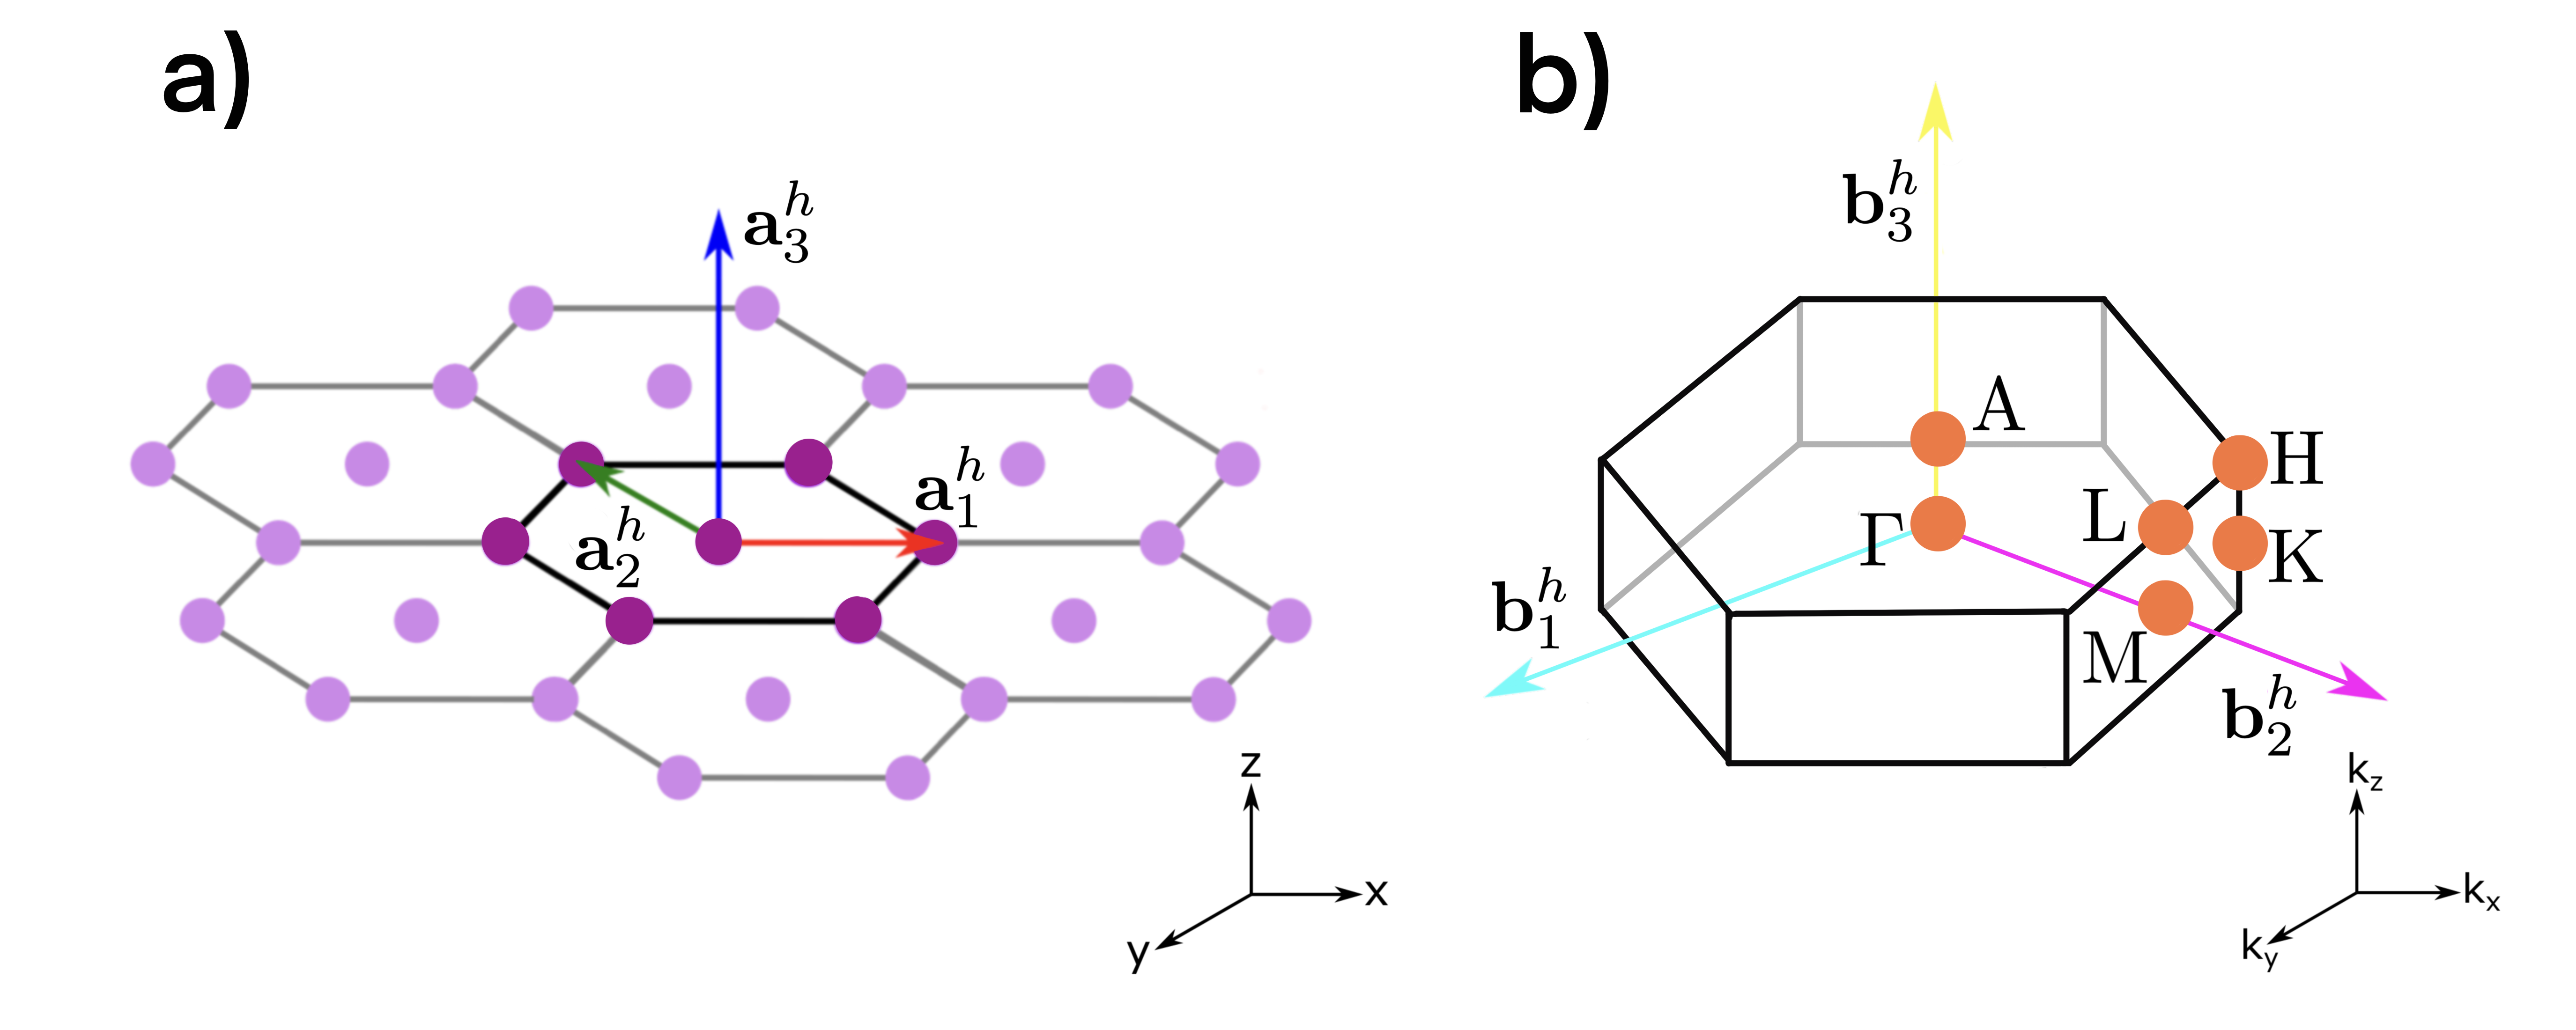
\includegraphics{./images/HexRealRec.png}

}

\caption{\label{fig-HexRealRec}a) Estructura de la celda unitaria para
el Hamiltoniano topológico de bismuto en el espacio real y b) recíproco.
Los vectores de la red real están etiquetados por \(\mathbf{a}^h_n\) y
los de la red recíproca por \(\mathbf{b}^h_n\) (\(n=1,2,3\)).}

\end{figure}

Este sistema consiste de una red hexagonal simple que preserva las
simetrías espaciales de la red de bismuto. Los vectores de esta red
hexagonal en el espacio real son:

\[
\begin{align} 
    \mathbf{a}_1^h = \left (a,0,0 \right ) \hspace{10mm}
    \mathbf{a}_2^h = \left ( -\frac{1}{2}a , \frac{\sqrt{3}}{2}a , 0 \right ) \hspace{10mm}
    \mathbf{a}_3^h = \left (             0 , 0,c \right ) 
\end{align}
\]

La 1ZB en el espacio recíproco también consiste de una celda hexagonal.
Además, las coordenadas relativas de algunos de los puntos de alta
simetría en ella son:

\[    
\Gamma = \left ( 0,0,0 \right )
\] \[
    \mathrm{M} = \left ( \frac{1}{2},0,0 \right ) 
\] \[
    \mathrm{K} = \left ( \frac{1}{3},\frac{1}{3},0 \right ) 
\] \[
    \mathrm{A} = \left ( 0,0, \frac{1}{2} \right )
\] \[
    \mathrm{L} = \left ( \frac{1}{2},0,\frac{1}{2} \right ) 
\] \[
    \mathrm{H} = \left ( \frac{1}{3},\frac{1}{3},\frac{1}{2} \right ).
\]

\bookmarksetup{startatroot}

\hypertarget{sec-hamiltonian}{%
\chapter{Hamiltoniano de amarre fuerte de
bismuto}\label{sec-hamiltonian}}

\[
\newcommand{\bk}{\boldsymbol{k}}
\newcommand{\baI}{\boldsymbol{a}_1}
\newcommand{\baII}{\boldsymbol{a}_2}
\newcommand{\baIII}{\boldsymbol{a}_3}
\]

En el año 2018, Schindler y colaboradores calcularon la estructura
electrónica a primeros principios del bulto de bismuto y obtuvieron una
brecha energética directa entre la banda de conducción y la de valencia
en cada punto del espacio \(\bk\). Debido a la presencia de esta brecha,
pudieron analizar la estructura electrónica del bismuto en el esquema de
la Química Cuántica Topológica \cite{Bradlyn2017} (la cual se basa en el
paradigma de la Representación de Bandas \cite{Cano2021}), y confirmaron
el carácter de aislante topológico de orden superior (HOTI) de este
material. Finalmente, propusieron un Hamiltoniano de amarre fuerte
topológicamente equivalente a un modelo realista de bismuto que facilita
la identificación de los estados de borde pues no contienen los estados
del bulto semimetálico. Además, al únicamente considerar 8 orbitales por
celda unitaria, las simulaciones de sistemas tridimensionales grandes
son computacionalmente realizables.

\hypertarget{expresiuxf3n-analuxedtica}{%
\section{Expresión analítica}\label{expresiuxf3n-analuxedtica}}

El modelo del Hamiltoniano de 8 bandas de amarre fuerte del bismuto
propuesto por Schindler y colaboradores \cite{Schindler2018} es:

\[
\begin{align}
    H_{\rm TB}^{Schin}(\bk) =
    \begin{pmatrix}
    H_{TB,I} (\bk) + \epsilon I & \delta M_{TB} (\bk)\\
    \delta M_{TB} (\bk)^\dagger & H_{TB,II} (\bk) - \epsilon I 
    \end{pmatrix}
\end{align}
\]

donde los términos de \(H_{TB,I} (\bk)\), \(H_{TB,II} (\bk)\) y
\(M_{TB} (\bk)\) tienen la forma:

\[
\begin{align}
    H_{TB,I} (\bk) &=
    \Gamma_1 \lbrace m_I(1+ \cos{\bk \cdot \baIII^h}) - t_I[\cos{\bk \cdot \baI^h} + \cos{\bk \cdot \baII^h} + \cos{\bk \cdot (\baI^h + \baII^h)}] \rbrace \nonumber \\ 
    & + \lambda_I [\Gamma_2 \sin{\bk \cdot \baI^h} + \Gamma_{2,1}^{I,I} \sin{\bk \cdot \baII^h} + \Gamma_{2,2}^{I,I} \sin{\bk \cdot (\baI^h+\baII^h)} + \Gamma_3 \sin \bk \cdot \baIII^h]
\end{align}
\]

\[
\begin{align}
    H_{TB,II} (\bk) &=
    \Gamma_1 \lbrace m_{II}(1+ \cos{\bk \cdot \baIII^h}) - t_{II}[\cos{\bk \cdot \baI^h} + \cos{\bk \cdot \baII^h} + \cos{\bk \cdot (\baI^h + \baII^h)}] \rbrace \nonumber \\ 
    & + \lambda_{II} [\Gamma_2 \sin{\bk \cdot \baI^h} + \Gamma_{2,1}^{II,II} \sin{\bk \cdot \baII^h} + \Gamma_{2,2}^{II,II} \sin{\bk \cdot (\baI^h+\baII^h)} + \Gamma_3 \sin \bk \cdot \baIII^h]
\end{align}
\]

\[
\begin{align}
    M_{TB} (\bk) &=
    \Gamma_2 [\sin{\bk \cdot \baI^h} + \sin{\bk \cdot (2\baI^h+\baII^h)}] + \Gamma_{2,1}^{I,II}[\sin{\bk \cdot \baII^h} + \sin{\bk \cdot (\baII^h-\baI^h)}] \nonumber \\
    &- \Gamma_{2,2}^{I,II}[\sin{\bk \cdot (\baI^h+\baII^h)}+\sin{\bk \cdot (\baI^h+2\baII^h)}]  - i\Gamma_5[\cos \bk \cdot \baI^h + \cos{\bk \cdot (2\baI^h+\baII^h)}] \nonumber \\
    &-i\Gamma_{5,1}^{I,II} [\cos{\bk \cdot \baII^h}+ \cos{\bk \cdot (\baII^h-\baI^h)}] -i\Gamma_{5,2}^{I,II}[\cos {\bk \cdot (\baI^h + \baII^h)}+\cos {\bk \cdot (\baI^h + 2\baII^h)}]
\end{align}
\]

\hypertarget{implementaciuxf3n-en-pythtb}{%
\section{Implementación en PythTB}\label{implementaciuxf3n-en-pythtb}}

\begin{Shaded}
\begin{Highlighting}[]
\ImportTok{from}\NormalTok{ pylab }\ImportTok{import} \OperatorTok{*}
\ImportTok{from}\NormalTok{ pythtb }\ImportTok{import} \OperatorTok{*}

\NormalTok{a1 }\OperatorTok{=}\NormalTok{ [   }\DecValTok{1}\NormalTok{,        }\DecValTok{0}\NormalTok{,}\DecValTok{0}\NormalTok{]}
\NormalTok{a2 }\OperatorTok{=}\NormalTok{ [}\OperatorTok{{-}}\DecValTok{1}\OperatorTok{/}\DecValTok{2}\NormalTok{,sqrt(}\DecValTok{3}\NormalTok{)}\OperatorTok{/}\DecValTok{2}\NormalTok{,}\DecValTok{0}\NormalTok{]}
\NormalTok{a3 }\OperatorTok{=}\NormalTok{ [   }\DecValTok{0}\NormalTok{,        }\DecValTok{0}\NormalTok{,}\DecValTok{1}\NormalTok{]}

\NormalTok{lat }\OperatorTok{=}\NormalTok{ [a1,a2,a3]}
\NormalTok{orb }\OperatorTok{=}\NormalTok{ [[}\DecValTok{0}\NormalTok{,}\DecValTok{0}\NormalTok{,}\DecValTok{1}\OperatorTok{/}\DecValTok{2}\NormalTok{],}
\NormalTok{       [}\DecValTok{0}\NormalTok{,}\DecValTok{0}\NormalTok{,}\DecValTok{1}\OperatorTok{/}\DecValTok{2}\NormalTok{],}
\NormalTok{       [}\DecValTok{0}\NormalTok{,}\DecValTok{0}\NormalTok{,}\DecValTok{1}\OperatorTok{/}\DecValTok{2}\NormalTok{],}
\NormalTok{       [}\DecValTok{0}\NormalTok{,}\DecValTok{0}\NormalTok{,}\DecValTok{1}\OperatorTok{/}\DecValTok{2}\NormalTok{],}
\NormalTok{       [}\DecValTok{0}\NormalTok{,}\DecValTok{0}\NormalTok{,}\DecValTok{1}\OperatorTok{/}\DecValTok{2}\NormalTok{],}
\NormalTok{       [}\DecValTok{0}\NormalTok{,}\DecValTok{0}\NormalTok{,}\DecValTok{1}\OperatorTok{/}\DecValTok{2}\NormalTok{],}
\NormalTok{       [}\DecValTok{0}\NormalTok{,}\DecValTok{0}\NormalTok{,}\DecValTok{1}\OperatorTok{/}\DecValTok{2}\NormalTok{],}
\NormalTok{       [}\DecValTok{0}\NormalTok{,}\DecValTok{0}\NormalTok{,}\DecValTok{1}\OperatorTok{/}\DecValTok{2}\NormalTok{]]}

\NormalTok{tI  }\OperatorTok{=} \DecValTok{1}\OperatorTok{;}\NormalTok{ tII }\OperatorTok{=} \DecValTok{1}
\NormalTok{mI  }\OperatorTok{=} \DecValTok{2}\OperatorTok{;}\NormalTok{ mII }\OperatorTok{=} \DecValTok{2}
\NormalTok{ϵ }\OperatorTok{=} \FloatTok{0.1}
\NormalTok{λI }\OperatorTok{=} \FloatTok{0.3}\OperatorTok{;}\NormalTok{ λII }\OperatorTok{=} \DecValTok{1}
\NormalTok{ƔII }\OperatorTok{=} \DecValTok{1}
\NormalTok{δ }\OperatorTok{=} \FloatTok{0.3}

\NormalTok{Bismuto }\OperatorTok{=}\NormalTok{ tb\_model(}\DecValTok{3}\NormalTok{,}\DecValTok{3}\NormalTok{,lat,orb)}
\end{Highlighting}
\end{Shaded}

\begin{Shaded}
\begin{Highlighting}[]
\CommentTok{\# [0,0]}
\NormalTok{Bismuto.set\_hop( }\OperatorTok{{-}}\NormalTok{tI}\OperatorTok{/}\DecValTok{2}\NormalTok{,}\DecValTok{0}\NormalTok{,}\DecValTok{0}\NormalTok{,[ }\DecValTok{1}\NormalTok{,}\DecValTok{0}\NormalTok{,}\DecValTok{0}\NormalTok{] ) }\CommentTok{\# cell = [ 1,0,0] {-}\textgreater{} e\^{}\{ik·[(cell)·(a1,a2,a3)]\}}
\NormalTok{Bismuto.set\_hop( }\OperatorTok{{-}}\NormalTok{tI}\OperatorTok{/}\DecValTok{2}\NormalTok{,}\DecValTok{0}\NormalTok{,}\DecValTok{0}\NormalTok{,[ }\DecValTok{0}\NormalTok{,}\DecValTok{1}\NormalTok{,}\DecValTok{0}\NormalTok{] ) }\CommentTok{\# cell = [ 0,1,0] {-}\textgreater{} e\^{}\{ik·[(cell)·(a1,a2,a3)]\}}
\NormalTok{Bismuto.set\_hop( }\OperatorTok{{-}}\NormalTok{tI}\OperatorTok{/}\DecValTok{2}\NormalTok{,}\DecValTok{0}\NormalTok{,}\DecValTok{0}\NormalTok{,[ }\DecValTok{1}\NormalTok{,}\DecValTok{1}\NormalTok{,}\DecValTok{0}\NormalTok{] ) }\CommentTok{\# cell = [ 1,1,0] {-}\textgreater{} e\^{}\{ik·[(cell)·(a1,a2,a3)]\}}

\NormalTok{Bismuto.set\_hop(  mI}\OperatorTok{/}\DecValTok{2}\NormalTok{,}\DecValTok{0}\NormalTok{,}\DecValTok{0}\NormalTok{,[ }\DecValTok{0}\NormalTok{,}\DecValTok{0}\NormalTok{,}\DecValTok{1}\NormalTok{] ) }\CommentTok{\# cell = [ 0,0,1] {-}\textgreater{} e\^{}\{ik·[(cell)·(a1,a2,a3)]\}}
\end{Highlighting}
\end{Shaded}

\begin{Shaded}
\begin{Highlighting}[]
\CommentTok{\# [0,2]}

\NormalTok{Bismuto.set\_hop( }\OperatorTok{{-}}\NormalTok{λI}\OperatorTok{/}\DecValTok{2}\NormalTok{,}\DecValTok{0}\NormalTok{,}\DecValTok{2}\NormalTok{,[}\DecValTok{0}\NormalTok{,}\DecValTok{0}\NormalTok{, }\DecValTok{1}\NormalTok{] ) }\CommentTok{\# cell = [ 0,0,1] {-}\textgreater{} e\^{}\{ik·[(cell)·(a1,a2,a3)]\}}
\NormalTok{Bismuto.set\_hop(  λI}\OperatorTok{/}\DecValTok{2}\NormalTok{,}\DecValTok{0}\NormalTok{,}\DecValTok{2}\NormalTok{,[}\DecValTok{0}\NormalTok{,}\DecValTok{0}\NormalTok{,}\OperatorTok{{-}}\DecValTok{1}\NormalTok{] ) }\CommentTok{\# cell = [ 0,0,{-}1] {-}\textgreater{} e\^{}\{ik·[(cell)·(a1,a2,a3)]\}}
\end{Highlighting}
\end{Shaded}

\begin{Shaded}
\begin{Highlighting}[]
\CommentTok{\# [0,3]}
\NormalTok{Bismuto.set\_hop(  λI}\OperatorTok{/}\NormalTok{(}\OtherTok{2J}\NormalTok{),}\DecValTok{0}\NormalTok{,}\DecValTok{3}\NormalTok{,[ }\DecValTok{1}\NormalTok{,}\DecValTok{0}\NormalTok{,}\DecValTok{0}\NormalTok{] ) }\CommentTok{\# cell = [ 1,0,0] {-}\textgreater{} e\^{}\{ik·[(cell)·(a1,a2,a3)]\}}
\NormalTok{Bismuto.set\_hop( }\OperatorTok{{-}}\NormalTok{λI}\OperatorTok{/}\NormalTok{(}\OtherTok{2J}\NormalTok{),}\DecValTok{0}\NormalTok{,}\DecValTok{3}\NormalTok{,[}\OperatorTok{{-}}\DecValTok{1}\NormalTok{,}\DecValTok{0}\NormalTok{,}\DecValTok{0}\NormalTok{] ) }\CommentTok{\# cell = [{-}1,0,0] {-}\textgreater{} e\^{}\{ik·[(cell)·(a1,a2,a3)]\}}
\NormalTok{Bismuto.set\_hop(  λI}\OperatorTok{/}\NormalTok{(}\OtherTok{2J}\NormalTok{)}\OperatorTok{*}\NormalTok{exp(}\OtherTok{2J}\OperatorTok{*}\NormalTok{pi}\OperatorTok{/}\DecValTok{3}\NormalTok{),}\DecValTok{0}\NormalTok{,}\DecValTok{3}\NormalTok{,[ }\DecValTok{0}\NormalTok{, }\DecValTok{1}\NormalTok{,}\DecValTok{0}\NormalTok{] ) }\CommentTok{\# cell = [ 0,1,0] {-}\textgreater{} e\^{}\{ik·[(cell)·(a1,a2,a3)]\}}
\NormalTok{Bismuto.set\_hop( }\OperatorTok{{-}}\NormalTok{λI}\OperatorTok{/}\NormalTok{(}\OtherTok{2J}\NormalTok{)}\OperatorTok{*}\NormalTok{exp(}\OtherTok{2J}\OperatorTok{*}\NormalTok{pi}\OperatorTok{/}\DecValTok{3}\NormalTok{),}\DecValTok{0}\NormalTok{,}\DecValTok{3}\NormalTok{,[ }\DecValTok{0}\NormalTok{,}\OperatorTok{{-}}\DecValTok{1}\NormalTok{,}\DecValTok{0}\NormalTok{] ) }\CommentTok{\# cell = [ 0,{-}1,0] {-}\textgreater{} e\^{}\{ik·[(cell)·(a1,a2,a3)]\}}
\NormalTok{Bismuto.set\_hop(  λI}\OperatorTok{/}\NormalTok{(}\OtherTok{2J}\NormalTok{)}\OperatorTok{*}\NormalTok{exp(}\OtherTok{1J}\OperatorTok{*}\NormalTok{pi}\OperatorTok{/}\DecValTok{3}\NormalTok{),}\DecValTok{0}\NormalTok{,}\DecValTok{3}\NormalTok{,[ }\DecValTok{1}\NormalTok{, }\DecValTok{1}\NormalTok{,}\DecValTok{0}\NormalTok{] ) }\CommentTok{\# cell = [ 1, 1,0] {-}\textgreater{} e\^{}\{ik·[(cell)·(a1,a2,a3)]\}}
\NormalTok{Bismuto.set\_hop( }\OperatorTok{{-}}\NormalTok{λI}\OperatorTok{/}\NormalTok{(}\OtherTok{2J}\NormalTok{)}\OperatorTok{*}\NormalTok{exp(}\OtherTok{1J}\OperatorTok{*}\NormalTok{pi}\OperatorTok{/}\DecValTok{3}\NormalTok{),}\DecValTok{0}\NormalTok{,}\DecValTok{3}\NormalTok{,[}\OperatorTok{{-}}\DecValTok{1}\NormalTok{,}\OperatorTok{{-}}\DecValTok{1}\NormalTok{,}\DecValTok{0}\NormalTok{] ) }\CommentTok{\# cell = [{-}1,{-}1,0] {-}\textgreater{} e\^{}\{ik·[(cell)·(a1,a2,a3)]\}}
\end{Highlighting}
\end{Shaded}

\begin{Shaded}
\begin{Highlighting}[]
\CommentTok{\# [0,5]}
\NormalTok{Bismuto.set\_hop(  }\OtherTok{1J}\OperatorTok{*}\NormalTok{δ}\OperatorTok{/}\DecValTok{2}\OperatorTok{*}\NormalTok{exp(}\OtherTok{1J}\OperatorTok{*}\NormalTok{pi}\OperatorTok{/}\DecValTok{3}\NormalTok{),}\DecValTok{0}\NormalTok{,}\DecValTok{5}\NormalTok{,[ }\DecValTok{0}\NormalTok{, }\DecValTok{1}\NormalTok{,}\DecValTok{0}\NormalTok{] ) }\CommentTok{\# cell = [ 0,1,0] {-}\textgreater{} e\^{}\{ik·[(cell)·(a1,a2,a3)]\}}
\NormalTok{Bismuto.set\_hop(  }\OtherTok{1J}\OperatorTok{*}\NormalTok{δ}\OperatorTok{/}\DecValTok{2}\OperatorTok{*}\NormalTok{exp(}\OtherTok{1J}\OperatorTok{*}\NormalTok{pi}\OperatorTok{/}\DecValTok{3}\NormalTok{),}\DecValTok{0}\NormalTok{,}\DecValTok{5}\NormalTok{,[ }\DecValTok{0}\NormalTok{,}\OperatorTok{{-}}\DecValTok{1}\NormalTok{,}\DecValTok{0}\NormalTok{] ) }\CommentTok{\# cell = [0,{-}1,0] {-}\textgreater{} e\^{}\{ik·[(cell)·(a1,a2,a3)]\}}
\NormalTok{Bismuto.set\_hop(  }\OtherTok{1J}\OperatorTok{*}\NormalTok{δ}\OperatorTok{/}\DecValTok{2}\OperatorTok{*}\NormalTok{exp(}\OtherTok{1J}\OperatorTok{*}\NormalTok{pi}\OperatorTok{/}\DecValTok{3}\NormalTok{),}\DecValTok{0}\NormalTok{,}\DecValTok{5}\NormalTok{,[}\OperatorTok{{-}}\DecValTok{1}\NormalTok{, }\DecValTok{1}\NormalTok{,}\DecValTok{0}\NormalTok{] ) }\CommentTok{\# cell = [{-}1,1,0] {-}\textgreater{} e\^{}\{ik·[(cell)·(a1,a2,a3)]\}}
\NormalTok{Bismuto.set\_hop(  }\OtherTok{1J}\OperatorTok{*}\NormalTok{δ}\OperatorTok{/}\DecValTok{2}\OperatorTok{*}\NormalTok{exp(}\OtherTok{1J}\OperatorTok{*}\NormalTok{pi}\OperatorTok{/}\DecValTok{3}\NormalTok{),}\DecValTok{0}\NormalTok{,}\DecValTok{5}\NormalTok{,[ }\DecValTok{1}\NormalTok{,}\OperatorTok{{-}}\DecValTok{1}\NormalTok{,}\DecValTok{0}\NormalTok{] ) }\CommentTok{\# cell = [1,{-}1,0] {-}\textgreater{} e\^{}\{ik·[(cell)·(a1,a2,a3)]\}}

\NormalTok{Bismuto.set\_hop( }\OperatorTok{{-}}\OtherTok{1J}\OperatorTok{*}\NormalTok{δ}\OperatorTok{/}\DecValTok{2}\NormalTok{,}\DecValTok{0}\NormalTok{,}\DecValTok{5}\NormalTok{,[ }\DecValTok{1}\NormalTok{, }\DecValTok{0}\NormalTok{,}\DecValTok{0}\NormalTok{] ) }\CommentTok{\# cell = [1,0,0] {-}\textgreater{} e\^{}\{ik·[(cell)·(a1,a2,a3)]\}}
\NormalTok{Bismuto.set\_hop( }\OperatorTok{{-}}\OtherTok{1J}\OperatorTok{*}\NormalTok{δ}\OperatorTok{/}\DecValTok{2}\NormalTok{,}\DecValTok{0}\NormalTok{,}\DecValTok{5}\NormalTok{,[}\OperatorTok{{-}}\DecValTok{1}\NormalTok{, }\DecValTok{0}\NormalTok{,}\DecValTok{0}\NormalTok{] ) }\CommentTok{\# cell = [{-}1,0,0] {-}\textgreater{} e\^{}\{ik·[(cell)·(a1,a2,a3)]\}}
\NormalTok{Bismuto.set\_hop( }\OperatorTok{{-}}\OtherTok{1J}\OperatorTok{*}\NormalTok{δ}\OperatorTok{/}\DecValTok{2}\NormalTok{,}\DecValTok{0}\NormalTok{,}\DecValTok{5}\NormalTok{,[ }\DecValTok{2}\NormalTok{, }\DecValTok{1}\NormalTok{,}\DecValTok{0}\NormalTok{] ) }\CommentTok{\# cell = [2,1,0] {-}\textgreater{} e\^{}\{ik·[(cell)·(a1,a2,a3)]\}}
\NormalTok{Bismuto.set\_hop( }\OperatorTok{{-}}\OtherTok{1J}\OperatorTok{*}\NormalTok{δ}\OperatorTok{/}\DecValTok{2}\NormalTok{,}\DecValTok{0}\NormalTok{,}\DecValTok{5}\NormalTok{,[}\OperatorTok{{-}}\DecValTok{2}\NormalTok{,}\OperatorTok{{-}}\DecValTok{1}\NormalTok{,}\DecValTok{0}\NormalTok{]) }\CommentTok{\# cell = [{-}2,{-}1,0] {-}\textgreater{} e\^{}\{ik·[(cell)·(a1,a2,a3)]\}}

\NormalTok{Bismuto.set\_hop( }\OperatorTok{{-}}\OtherTok{1J}\OperatorTok{*}\NormalTok{δ}\OperatorTok{/}\DecValTok{2}\OperatorTok{*}\NormalTok{exp(}\OtherTok{2J}\OperatorTok{*}\NormalTok{pi}\OperatorTok{/}\DecValTok{3}\NormalTok{),}\DecValTok{0}\NormalTok{,}\DecValTok{5}\NormalTok{,[ }\DecValTok{1}\NormalTok{, }\DecValTok{1}\NormalTok{,}\DecValTok{0}\NormalTok{] ) }\CommentTok{\# cell = [1,0,0] {-}\textgreater{} e\^{}\{ik·[(cell)·(a1,a2,a3)]\}}
\NormalTok{Bismuto.set\_hop( }\OperatorTok{{-}}\OtherTok{1J}\OperatorTok{*}\NormalTok{δ}\OperatorTok{/}\DecValTok{2}\OperatorTok{*}\NormalTok{exp(}\OtherTok{2J}\OperatorTok{*}\NormalTok{pi}\OperatorTok{/}\DecValTok{3}\NormalTok{),}\DecValTok{0}\NormalTok{,}\DecValTok{5}\NormalTok{,[}\OperatorTok{{-}}\DecValTok{1}\NormalTok{,}\OperatorTok{{-}}\DecValTok{1}\NormalTok{,}\DecValTok{0}\NormalTok{] ) }\CommentTok{\# cell = [{-}1,0,0] {-}\textgreater{} e\^{}\{ik·[(cell)·(a1,a2,a3)]\}}
\NormalTok{Bismuto.set\_hop( }\OperatorTok{{-}}\OtherTok{1J}\OperatorTok{*}\NormalTok{δ}\OperatorTok{/}\DecValTok{2}\OperatorTok{*}\NormalTok{exp(}\OtherTok{2J}\OperatorTok{*}\NormalTok{pi}\OperatorTok{/}\DecValTok{3}\NormalTok{),}\DecValTok{0}\NormalTok{,}\DecValTok{5}\NormalTok{,[ }\DecValTok{1}\NormalTok{, }\DecValTok{2}\NormalTok{,}\DecValTok{0}\NormalTok{] ) }\CommentTok{\# cell = [2,1,0] {-}\textgreater{} e\^{}\{ik·[(cell)·(a1,a2,a3)]\}}
\NormalTok{Bismuto.set\_hop( }\OperatorTok{{-}}\OtherTok{1J}\OperatorTok{*}\NormalTok{δ}\OperatorTok{/}\DecValTok{2}\OperatorTok{*}\NormalTok{exp(}\OtherTok{2J}\OperatorTok{*}\NormalTok{pi}\OperatorTok{/}\DecValTok{3}\NormalTok{),}\DecValTok{0}\NormalTok{,}\DecValTok{5}\NormalTok{,[}\OperatorTok{{-}}\DecValTok{1}\NormalTok{,}\OperatorTok{{-}}\DecValTok{2}\NormalTok{,}\DecValTok{0}\NormalTok{]) }\CommentTok{\# cell = [{-}2,{-}1,0] {-}\textgreater{} e\^{}\{ik·[(cell)·(a1,a2,a3)]\}}
\end{Highlighting}
\end{Shaded}

\begin{Shaded}
\begin{Highlighting}[]
\CommentTok{\# [0,7]}
\NormalTok{Bismuto.set\_hop(  δ}\OperatorTok{/}\OtherTok{2J}\NormalTok{,}\DecValTok{0}\NormalTok{,}\DecValTok{7}\NormalTok{,[ }\DecValTok{1}\NormalTok{,}\DecValTok{0}\NormalTok{,}\DecValTok{0}\NormalTok{] ) }
\NormalTok{Bismuto.set\_hop( }\OperatorTok{{-}}\NormalTok{δ}\OperatorTok{/}\OtherTok{2J}\NormalTok{,}\DecValTok{0}\NormalTok{,}\DecValTok{7}\NormalTok{,[}\OperatorTok{{-}}\DecValTok{1}\NormalTok{,}\DecValTok{0}\NormalTok{,}\DecValTok{0}\NormalTok{] )}

\NormalTok{Bismuto.set\_hop( }\OperatorTok{{-}}\NormalTok{δ}\OperatorTok{/}\OtherTok{2J}\OperatorTok{*}\NormalTok{exp(}\OtherTok{1J}\OperatorTok{*}\NormalTok{pi}\OperatorTok{/}\DecValTok{3}\NormalTok{),}\DecValTok{0}\NormalTok{,}\DecValTok{7}\NormalTok{,[ }\DecValTok{0}\NormalTok{, }\DecValTok{1}\NormalTok{,}\DecValTok{0}\NormalTok{] ) }
\NormalTok{Bismuto.set\_hop(  δ}\OperatorTok{/}\OtherTok{2J}\OperatorTok{*}\NormalTok{exp(}\OtherTok{1J}\OperatorTok{*}\NormalTok{pi}\OperatorTok{/}\DecValTok{3}\NormalTok{),}\DecValTok{0}\NormalTok{,}\DecValTok{7}\NormalTok{,[ }\DecValTok{0}\NormalTok{,}\OperatorTok{{-}}\DecValTok{1}\NormalTok{,}\DecValTok{0}\NormalTok{] ) }
\NormalTok{Bismuto.set\_hop( }\OperatorTok{{-}}\NormalTok{δ}\OperatorTok{/}\OtherTok{2J}\OperatorTok{*}\NormalTok{exp(}\OtherTok{1J}\OperatorTok{*}\NormalTok{pi}\OperatorTok{/}\DecValTok{3}\NormalTok{),}\DecValTok{0}\NormalTok{,}\DecValTok{7}\NormalTok{,[}\OperatorTok{{-}}\DecValTok{1}\NormalTok{, }\DecValTok{1}\NormalTok{,}\DecValTok{0}\NormalTok{] ) }
\NormalTok{Bismuto.set\_hop(  δ}\OperatorTok{/}\OtherTok{2J}\OperatorTok{*}\NormalTok{exp(}\OtherTok{1J}\OperatorTok{*}\NormalTok{pi}\OperatorTok{/}\DecValTok{3}\NormalTok{),}\DecValTok{0}\NormalTok{,}\DecValTok{7}\NormalTok{,[ }\DecValTok{1}\NormalTok{,}\OperatorTok{{-}}\DecValTok{1}\NormalTok{,}\DecValTok{0}\NormalTok{] ) }

\NormalTok{Bismuto.set\_hop(  δ}\OperatorTok{/}\OtherTok{2J}\NormalTok{,}\DecValTok{0}\NormalTok{,}\DecValTok{7}\NormalTok{,[ }\DecValTok{2}\NormalTok{, }\DecValTok{1}\NormalTok{,}\DecValTok{0}\NormalTok{] ) }
\NormalTok{Bismuto.set\_hop( }\OperatorTok{{-}}\NormalTok{δ}\OperatorTok{/}\OtherTok{2J}\NormalTok{,}\DecValTok{0}\NormalTok{,}\DecValTok{7}\NormalTok{,[}\OperatorTok{{-}}\DecValTok{2}\NormalTok{,}\OperatorTok{{-}}\DecValTok{1}\NormalTok{,}\DecValTok{0}\NormalTok{] )}

\NormalTok{Bismuto.set\_hop( }\OperatorTok{{-}}\NormalTok{δ}\OperatorTok{/}\OtherTok{2J}\OperatorTok{*}\NormalTok{exp(}\OtherTok{2J}\OperatorTok{*}\NormalTok{pi}\OperatorTok{/}\DecValTok{3}\NormalTok{),}\DecValTok{0}\NormalTok{,}\DecValTok{7}\NormalTok{,[ }\DecValTok{1}\NormalTok{, }\DecValTok{1}\NormalTok{,}\DecValTok{0}\NormalTok{] ) }
\NormalTok{Bismuto.set\_hop(  δ}\OperatorTok{/}\OtherTok{2J}\OperatorTok{*}\NormalTok{exp(}\OtherTok{2J}\OperatorTok{*}\NormalTok{pi}\OperatorTok{/}\DecValTok{3}\NormalTok{),}\DecValTok{0}\NormalTok{,}\DecValTok{7}\NormalTok{,[}\OperatorTok{{-}}\DecValTok{1}\NormalTok{,}\OperatorTok{{-}}\DecValTok{1}\NormalTok{,}\DecValTok{0}\NormalTok{] ) }
\NormalTok{Bismuto.set\_hop( }\OperatorTok{{-}}\NormalTok{δ}\OperatorTok{/}\OtherTok{2J}\OperatorTok{*}\NormalTok{exp(}\OtherTok{2J}\OperatorTok{*}\NormalTok{pi}\OperatorTok{/}\DecValTok{3}\NormalTok{),}\DecValTok{0}\NormalTok{,}\DecValTok{7}\NormalTok{,[ }\DecValTok{1}\NormalTok{, }\DecValTok{2}\NormalTok{,}\DecValTok{0}\NormalTok{] ) }
\NormalTok{Bismuto.set\_hop(  δ}\OperatorTok{/}\OtherTok{2J}\OperatorTok{*}\NormalTok{exp(}\OtherTok{2J}\OperatorTok{*}\NormalTok{pi}\OperatorTok{/}\DecValTok{3}\NormalTok{),}\DecValTok{0}\NormalTok{,}\DecValTok{7}\NormalTok{,[}\OperatorTok{{-}}\DecValTok{1}\NormalTok{,}\OperatorTok{{-}}\DecValTok{2}\NormalTok{,}\DecValTok{0}\NormalTok{] ) }
\end{Highlighting}
\end{Shaded}

\begin{Shaded}
\begin{Highlighting}[]
\CommentTok{\# [1,1]}
\NormalTok{Bismuto.set\_hop( }\OperatorTok{{-}}\NormalTok{tI}\OperatorTok{/}\DecValTok{2}\NormalTok{,}\DecValTok{1}\NormalTok{,}\DecValTok{1}\NormalTok{,[  }\DecValTok{1}\NormalTok{, }\DecValTok{0}\NormalTok{,}\DecValTok{0}\NormalTok{] ) }
\CommentTok{\#Bismuto.set\_hop( {-}tI/2,1,1,[ {-}1, 0,0] ) }
\NormalTok{Bismuto.set\_hop( }\OperatorTok{{-}}\NormalTok{tI}\OperatorTok{/}\DecValTok{2}\NormalTok{,}\DecValTok{1}\NormalTok{,}\DecValTok{1}\NormalTok{,[  }\DecValTok{0}\NormalTok{, }\DecValTok{1}\NormalTok{,}\DecValTok{0}\NormalTok{] ) }
\CommentTok{\#Bismuto.set\_hop( {-}tI/2,1,1,[  0,{-}1,0] ) }
\NormalTok{Bismuto.set\_hop( }\OperatorTok{{-}}\NormalTok{tI}\OperatorTok{/}\DecValTok{2}\NormalTok{,}\DecValTok{1}\NormalTok{,}\DecValTok{1}\NormalTok{,[  }\DecValTok{1}\NormalTok{, }\DecValTok{1}\NormalTok{,}\DecValTok{0}\NormalTok{] ) }
\CommentTok{\#Bismuto.set\_hop( {-}tI/2,1,1,[ {-}1,{-}1,0] ) }

\NormalTok{Bismuto.set\_hop( mI}\OperatorTok{/}\DecValTok{2}\NormalTok{,}\DecValTok{1}\NormalTok{,}\DecValTok{1}\NormalTok{,[ }\DecValTok{0}\NormalTok{,}\DecValTok{0}\NormalTok{, }\DecValTok{1}\NormalTok{] ) }
\CommentTok{\#Bismuto.set\_hop( mI/2,1,1,[ 0,0,{-}1] ) }
\end{Highlighting}
\end{Shaded}

\begin{Shaded}
\begin{Highlighting}[]
\CommentTok{\# [1,2]}
\NormalTok{Bismuto.set\_hop(  λI}\OperatorTok{/}\NormalTok{(}\OtherTok{2J}\NormalTok{),}\DecValTok{1}\NormalTok{,}\DecValTok{2}\NormalTok{,[ }\DecValTok{1}\NormalTok{,}\DecValTok{0}\NormalTok{,}\DecValTok{0}\NormalTok{] ) }
\NormalTok{Bismuto.set\_hop( }\OperatorTok{{-}}\NormalTok{λI}\OperatorTok{/}\NormalTok{(}\OtherTok{2J}\NormalTok{),}\DecValTok{1}\NormalTok{,}\DecValTok{2}\NormalTok{,[}\OperatorTok{{-}}\DecValTok{1}\NormalTok{,}\DecValTok{0}\NormalTok{,}\DecValTok{0}\NormalTok{] ) }

\NormalTok{Bismuto.set\_hop(  λI}\OperatorTok{/}\NormalTok{(}\OtherTok{2J}\NormalTok{)}\OperatorTok{*}\NormalTok{exp(}\OperatorTok{{-}}\OtherTok{2J}\OperatorTok{*}\NormalTok{pi}\OperatorTok{/}\DecValTok{3}\NormalTok{),}\DecValTok{1}\NormalTok{,}\DecValTok{2}\NormalTok{,[}\DecValTok{0}\NormalTok{, }\DecValTok{1}\NormalTok{,}\DecValTok{0}\NormalTok{] ) }
\NormalTok{Bismuto.set\_hop( }\OperatorTok{{-}}\NormalTok{λI}\OperatorTok{/}\NormalTok{(}\OtherTok{2J}\NormalTok{)}\OperatorTok{*}\NormalTok{exp(}\OperatorTok{{-}}\OtherTok{2J}\OperatorTok{*}\NormalTok{pi}\OperatorTok{/}\DecValTok{3}\NormalTok{),}\DecValTok{1}\NormalTok{,}\DecValTok{2}\NormalTok{,[}\DecValTok{0}\NormalTok{,}\OperatorTok{{-}}\DecValTok{1}\NormalTok{,}\DecValTok{0}\NormalTok{] ) }

\NormalTok{Bismuto.set\_hop(  λI}\OperatorTok{/}\NormalTok{(}\OtherTok{2J}\NormalTok{)}\OperatorTok{*}\NormalTok{exp(}\OperatorTok{{-}}\OtherTok{1J}\OperatorTok{*}\NormalTok{pi}\OperatorTok{/}\DecValTok{3}\NormalTok{),}\DecValTok{1}\NormalTok{,}\DecValTok{2}\NormalTok{,[ }\DecValTok{1}\NormalTok{, }\DecValTok{1}\NormalTok{,}\DecValTok{0}\NormalTok{] ) }
\NormalTok{Bismuto.set\_hop( }\OperatorTok{{-}}\NormalTok{λI}\OperatorTok{/}\NormalTok{(}\OtherTok{2J}\NormalTok{)}\OperatorTok{*}\NormalTok{exp(}\OperatorTok{{-}}\OtherTok{1J}\OperatorTok{*}\NormalTok{pi}\OperatorTok{/}\DecValTok{3}\NormalTok{),}\DecValTok{1}\NormalTok{,}\DecValTok{2}\NormalTok{,[}\OperatorTok{{-}}\DecValTok{1}\NormalTok{,}\OperatorTok{{-}}\DecValTok{1}\NormalTok{,}\DecValTok{0}\NormalTok{] ) }
\end{Highlighting}
\end{Shaded}

\begin{Shaded}
\begin{Highlighting}[]
\CommentTok{\#[1,3]}
\NormalTok{Bismuto.set\_hop( }\OperatorTok{{-}}\NormalTok{λI}\OperatorTok{/}\DecValTok{2}\NormalTok{,}\DecValTok{1}\NormalTok{,}\DecValTok{3}\NormalTok{,[ }\DecValTok{0}\NormalTok{,}\DecValTok{0}\NormalTok{, }\DecValTok{1}\NormalTok{] ) }
\NormalTok{Bismuto.set\_hop(  λI}\OperatorTok{/}\DecValTok{2}\NormalTok{,}\DecValTok{1}\NormalTok{,}\DecValTok{3}\NormalTok{,[ }\DecValTok{0}\NormalTok{,}\DecValTok{0}\NormalTok{,}\OperatorTok{{-}}\DecValTok{1}\NormalTok{] ) }
\end{Highlighting}
\end{Shaded}

\begin{Shaded}
\begin{Highlighting}[]
\CommentTok{\#[1,4]}
\NormalTok{Bismuto.set\_hop(  }\OtherTok{1J}\OperatorTok{*}\NormalTok{δ}\OperatorTok{/}\DecValTok{2}\OperatorTok{*}\NormalTok{exp(}\OperatorTok{{-}}\OtherTok{1J}\OperatorTok{*}\NormalTok{pi}\OperatorTok{/}\DecValTok{3}\NormalTok{),}\DecValTok{1}\NormalTok{,}\DecValTok{4}\NormalTok{,[  }\DecValTok{0}\NormalTok{, }\DecValTok{1}\NormalTok{,}\DecValTok{0}\NormalTok{] ) }
\NormalTok{Bismuto.set\_hop(  }\OtherTok{1J}\OperatorTok{*}\NormalTok{δ}\OperatorTok{/}\DecValTok{2}\OperatorTok{*}\NormalTok{exp(}\OperatorTok{{-}}\OtherTok{1J}\OperatorTok{*}\NormalTok{pi}\OperatorTok{/}\DecValTok{3}\NormalTok{),}\DecValTok{1}\NormalTok{,}\DecValTok{4}\NormalTok{,[  }\DecValTok{0}\NormalTok{,}\OperatorTok{{-}}\DecValTok{1}\NormalTok{,}\DecValTok{0}\NormalTok{] )}
\NormalTok{Bismuto.set\_hop(  }\OtherTok{1J}\OperatorTok{*}\NormalTok{δ}\OperatorTok{/}\DecValTok{2}\OperatorTok{*}\NormalTok{exp(}\OperatorTok{{-}}\OtherTok{1J}\OperatorTok{*}\NormalTok{pi}\OperatorTok{/}\DecValTok{3}\NormalTok{),}\DecValTok{1}\NormalTok{,}\DecValTok{4}\NormalTok{,[ }\OperatorTok{{-}}\DecValTok{1}\NormalTok{, }\DecValTok{1}\NormalTok{,}\DecValTok{0}\NormalTok{] )  }
\NormalTok{Bismuto.set\_hop(  }\OtherTok{1J}\OperatorTok{*}\NormalTok{δ}\OperatorTok{/}\DecValTok{2}\OperatorTok{*}\NormalTok{exp(}\OperatorTok{{-}}\OtherTok{1J}\OperatorTok{*}\NormalTok{pi}\OperatorTok{/}\DecValTok{3}\NormalTok{),}\DecValTok{1}\NormalTok{,}\DecValTok{4}\NormalTok{,[  }\DecValTok{1}\NormalTok{,}\OperatorTok{{-}}\DecValTok{1}\NormalTok{,}\DecValTok{0}\NormalTok{] ) }

\NormalTok{Bismuto.set\_hop( }\OperatorTok{{-}}\OtherTok{1J}\OperatorTok{*}\NormalTok{δ}\OperatorTok{/}\DecValTok{2}\NormalTok{,}\DecValTok{1}\NormalTok{,}\DecValTok{4}\NormalTok{,[  }\DecValTok{1}\NormalTok{, }\DecValTok{0}\NormalTok{,}\DecValTok{0}\NormalTok{] ) }
\NormalTok{Bismuto.set\_hop( }\OperatorTok{{-}}\OtherTok{1J}\OperatorTok{*}\NormalTok{δ}\OperatorTok{/}\DecValTok{2}\NormalTok{,}\DecValTok{1}\NormalTok{,}\DecValTok{4}\NormalTok{,[ }\OperatorTok{{-}}\DecValTok{1}\NormalTok{, }\DecValTok{0}\NormalTok{,}\DecValTok{0}\NormalTok{] )}
\NormalTok{Bismuto.set\_hop( }\OperatorTok{{-}}\OtherTok{1J}\OperatorTok{*}\NormalTok{δ}\OperatorTok{/}\DecValTok{2}\NormalTok{,}\DecValTok{1}\NormalTok{,}\DecValTok{4}\NormalTok{,[  }\DecValTok{2}\NormalTok{, }\DecValTok{1}\NormalTok{,}\DecValTok{0}\NormalTok{] )  }
\NormalTok{Bismuto.set\_hop( }\OperatorTok{{-}}\OtherTok{1J}\OperatorTok{*}\NormalTok{δ}\OperatorTok{/}\DecValTok{2}\NormalTok{,}\DecValTok{1}\NormalTok{,}\DecValTok{4}\NormalTok{,[ }\OperatorTok{{-}}\DecValTok{2}\NormalTok{,}\OperatorTok{{-}}\DecValTok{1}\NormalTok{,}\DecValTok{0}\NormalTok{] ) }

\NormalTok{Bismuto.set\_hop( }\OperatorTok{{-}}\OtherTok{1J}\OperatorTok{*}\NormalTok{δ}\OperatorTok{/}\DecValTok{2}\OperatorTok{*}\NormalTok{exp(}\OperatorTok{{-}}\OtherTok{2J}\OperatorTok{*}\NormalTok{pi}\OperatorTok{/}\DecValTok{3}\NormalTok{),}\DecValTok{1}\NormalTok{,}\DecValTok{4}\NormalTok{,[  }\DecValTok{1}\NormalTok{, }\DecValTok{1}\NormalTok{,}\DecValTok{0}\NormalTok{] ) }
\NormalTok{Bismuto.set\_hop( }\OperatorTok{{-}}\OtherTok{1J}\OperatorTok{*}\NormalTok{δ}\OperatorTok{/}\DecValTok{2}\OperatorTok{*}\NormalTok{exp(}\OperatorTok{{-}}\OtherTok{2J}\OperatorTok{*}\NormalTok{pi}\OperatorTok{/}\DecValTok{3}\NormalTok{),}\DecValTok{1}\NormalTok{,}\DecValTok{4}\NormalTok{,[ }\OperatorTok{{-}}\DecValTok{1}\NormalTok{,}\OperatorTok{{-}}\DecValTok{1}\NormalTok{,}\DecValTok{0}\NormalTok{] )}
\NormalTok{Bismuto.set\_hop( }\OperatorTok{{-}}\OtherTok{1J}\OperatorTok{*}\NormalTok{δ}\OperatorTok{/}\DecValTok{2}\OperatorTok{*}\NormalTok{exp(}\OperatorTok{{-}}\OtherTok{2J}\OperatorTok{*}\NormalTok{pi}\OperatorTok{/}\DecValTok{3}\NormalTok{),}\DecValTok{1}\NormalTok{,}\DecValTok{4}\NormalTok{,[  }\DecValTok{1}\NormalTok{, }\DecValTok{2}\NormalTok{,}\DecValTok{0}\NormalTok{] )  }
\NormalTok{Bismuto.set\_hop( }\OperatorTok{{-}}\OtherTok{1J}\OperatorTok{*}\NormalTok{δ}\OperatorTok{/}\DecValTok{2}\OperatorTok{*}\NormalTok{exp(}\OperatorTok{{-}}\OtherTok{2J}\OperatorTok{*}\NormalTok{pi}\OperatorTok{/}\DecValTok{3}\NormalTok{),}\DecValTok{1}\NormalTok{,}\DecValTok{4}\NormalTok{,[ }\OperatorTok{{-}}\DecValTok{1}\NormalTok{,}\OperatorTok{{-}}\DecValTok{2}\NormalTok{,}\DecValTok{0}\NormalTok{] ) }
\end{Highlighting}
\end{Shaded}

\begin{Shaded}
\begin{Highlighting}[]
\CommentTok{\#[1,6]}
\NormalTok{Bismuto.set\_hop(   δ}\OperatorTok{/}\OtherTok{2J}\NormalTok{,}\DecValTok{1}\NormalTok{,}\DecValTok{6}\NormalTok{,[  }\DecValTok{1}\NormalTok{,}\DecValTok{0}\NormalTok{,}\DecValTok{0}\NormalTok{] ) }
\NormalTok{Bismuto.set\_hop(  }\OperatorTok{{-}}\NormalTok{δ}\OperatorTok{/}\OtherTok{2J}\NormalTok{,}\DecValTok{1}\NormalTok{,}\DecValTok{6}\NormalTok{,[ }\OperatorTok{{-}}\DecValTok{1}\NormalTok{,}\DecValTok{0}\NormalTok{,}\DecValTok{0}\NormalTok{] )}

\NormalTok{Bismuto.set\_hop(  }\OperatorTok{{-}}\NormalTok{δ}\OperatorTok{/}\OtherTok{2J}\OperatorTok{*}\NormalTok{exp(}\OperatorTok{{-}}\OtherTok{1J}\OperatorTok{*}\NormalTok{pi}\OperatorTok{/}\DecValTok{3}\NormalTok{),}\DecValTok{1}\NormalTok{,}\DecValTok{6}\NormalTok{,[  }\DecValTok{0}\NormalTok{, }\DecValTok{1}\NormalTok{,}\DecValTok{0}\NormalTok{] )  }
\NormalTok{Bismuto.set\_hop(   δ}\OperatorTok{/}\OtherTok{2J}\OperatorTok{*}\NormalTok{exp(}\OperatorTok{{-}}\OtherTok{1J}\OperatorTok{*}\NormalTok{pi}\OperatorTok{/}\DecValTok{3}\NormalTok{),}\DecValTok{1}\NormalTok{,}\DecValTok{6}\NormalTok{,[  }\DecValTok{0}\NormalTok{,}\OperatorTok{{-}}\DecValTok{1}\NormalTok{,}\DecValTok{0}\NormalTok{] ) }
\NormalTok{Bismuto.set\_hop(  }\OperatorTok{{-}}\NormalTok{δ}\OperatorTok{/}\OtherTok{2J}\OperatorTok{*}\NormalTok{exp(}\OperatorTok{{-}}\OtherTok{1J}\OperatorTok{*}\NormalTok{pi}\OperatorTok{/}\DecValTok{3}\NormalTok{),}\DecValTok{1}\NormalTok{,}\DecValTok{6}\NormalTok{,[ }\OperatorTok{{-}}\DecValTok{1}\NormalTok{, }\DecValTok{1}\NormalTok{,}\DecValTok{0}\NormalTok{] )  }
\NormalTok{Bismuto.set\_hop(   δ}\OperatorTok{/}\OtherTok{2J}\OperatorTok{*}\NormalTok{exp(}\OperatorTok{{-}}\OtherTok{1J}\OperatorTok{*}\NormalTok{pi}\OperatorTok{/}\DecValTok{3}\NormalTok{),}\DecValTok{1}\NormalTok{,}\DecValTok{6}\NormalTok{,[  }\DecValTok{1}\NormalTok{,}\OperatorTok{{-}}\DecValTok{1}\NormalTok{,}\DecValTok{0}\NormalTok{] )}

\NormalTok{Bismuto.set\_hop(   δ}\OperatorTok{/}\OtherTok{2J}\NormalTok{,}\DecValTok{1}\NormalTok{,}\DecValTok{6}\NormalTok{,[  }\DecValTok{2}\NormalTok{, }\DecValTok{1}\NormalTok{,}\DecValTok{0}\NormalTok{] ) }
\NormalTok{Bismuto.set\_hop(  }\OperatorTok{{-}}\NormalTok{δ}\OperatorTok{/}\OtherTok{2J}\NormalTok{,}\DecValTok{1}\NormalTok{,}\DecValTok{6}\NormalTok{,[ }\OperatorTok{{-}}\DecValTok{2}\NormalTok{,}\OperatorTok{{-}}\DecValTok{1}\NormalTok{,}\DecValTok{0}\NormalTok{] )}

\NormalTok{Bismuto.set\_hop(  }\OperatorTok{{-}}\NormalTok{δ}\OperatorTok{/}\OtherTok{2J}\OperatorTok{*}\NormalTok{exp(}\OperatorTok{{-}}\OtherTok{2J}\OperatorTok{*}\NormalTok{pi}\OperatorTok{/}\DecValTok{3}\NormalTok{),}\DecValTok{1}\NormalTok{,}\DecValTok{6}\NormalTok{,[  }\DecValTok{1}\NormalTok{, }\DecValTok{1}\NormalTok{,}\DecValTok{0}\NormalTok{] )  }
\NormalTok{Bismuto.set\_hop(   δ}\OperatorTok{/}\OtherTok{2J}\OperatorTok{*}\NormalTok{exp(}\OperatorTok{{-}}\OtherTok{2J}\OperatorTok{*}\NormalTok{pi}\OperatorTok{/}\DecValTok{3}\NormalTok{),}\DecValTok{1}\NormalTok{,}\DecValTok{6}\NormalTok{,[ }\OperatorTok{{-}}\DecValTok{1}\NormalTok{,}\OperatorTok{{-}}\DecValTok{1}\NormalTok{,}\DecValTok{0}\NormalTok{] ) }
\NormalTok{Bismuto.set\_hop(  }\OperatorTok{{-}}\NormalTok{δ}\OperatorTok{/}\OtherTok{2J}\OperatorTok{*}\NormalTok{exp(}\OperatorTok{{-}}\OtherTok{2J}\OperatorTok{*}\NormalTok{pi}\OperatorTok{/}\DecValTok{3}\NormalTok{),}\DecValTok{1}\NormalTok{,}\DecValTok{6}\NormalTok{,[  }\DecValTok{1}\NormalTok{, }\DecValTok{2}\NormalTok{,}\DecValTok{0}\NormalTok{] )  }
\NormalTok{Bismuto.set\_hop(   δ}\OperatorTok{/}\OtherTok{2J}\OperatorTok{*}\NormalTok{exp(}\OperatorTok{{-}}\OtherTok{2J}\OperatorTok{*}\NormalTok{pi}\OperatorTok{/}\DecValTok{3}\NormalTok{),}\DecValTok{1}\NormalTok{,}\DecValTok{6}\NormalTok{,[ }\OperatorTok{{-}}\DecValTok{1}\NormalTok{,}\OperatorTok{{-}}\DecValTok{2}\NormalTok{,}\DecValTok{0}\NormalTok{] )}
\end{Highlighting}
\end{Shaded}

\begin{Shaded}
\begin{Highlighting}[]
\CommentTok{\#[2,2]}
\NormalTok{Bismuto.set\_hop( tI}\OperatorTok{/}\DecValTok{2}\NormalTok{,}\DecValTok{2}\NormalTok{,}\DecValTok{2}\NormalTok{,[  }\DecValTok{1}\NormalTok{,}\DecValTok{0}\NormalTok{,}\DecValTok{0}\NormalTok{] ) }
\CommentTok{\#Bismuto.set\_hop( {-}tI/2,2,2,[ {-}1,0,0] ) }
\NormalTok{Bismuto.set\_hop( tI}\OperatorTok{/}\DecValTok{2}\NormalTok{,}\DecValTok{2}\NormalTok{,}\DecValTok{2}\NormalTok{,[ }\DecValTok{0}\NormalTok{, }\DecValTok{1}\NormalTok{,}\DecValTok{0}\NormalTok{] ) }
\CommentTok{\#Bismuto.set\_hop( {-}tI/2,2,2,[ 0,{-}1,0] ) }
\NormalTok{Bismuto.set\_hop( tI}\OperatorTok{/}\DecValTok{2}\NormalTok{,}\DecValTok{2}\NormalTok{,}\DecValTok{2}\NormalTok{,[  }\DecValTok{1}\NormalTok{, }\DecValTok{1}\NormalTok{,}\DecValTok{0}\NormalTok{] )}
\CommentTok{\#Bismuto.set\_hop( {-}tI/2,2,2,[ {-}1,{-}1,0] ) }

\NormalTok{Bismuto.set\_hop( }\OperatorTok{{-}}\NormalTok{mI}\OperatorTok{/}\DecValTok{2}\NormalTok{,}\DecValTok{2}\NormalTok{,}\DecValTok{2}\NormalTok{,[ }\DecValTok{0}\NormalTok{,}\DecValTok{0}\NormalTok{, }\DecValTok{1}\NormalTok{] ) }
\CommentTok{\#Bismuto.set\_hop( {-}mI/2,2,2,[ 0,0,{-}1] ) }
\end{Highlighting}
\end{Shaded}

\begin{Shaded}
\begin{Highlighting}[]
\CommentTok{\#[2,5]}
\NormalTok{Bismuto.set\_hop(   δ}\OperatorTok{/}\OtherTok{2J}\NormalTok{,}\DecValTok{2}\NormalTok{,}\DecValTok{5}\NormalTok{,[  }\DecValTok{1}\NormalTok{,}\DecValTok{0}\NormalTok{,}\DecValTok{0}\NormalTok{] ) }
\NormalTok{Bismuto.set\_hop(  }\OperatorTok{{-}}\NormalTok{δ}\OperatorTok{/}\OtherTok{2J}\NormalTok{,}\DecValTok{2}\NormalTok{,}\DecValTok{5}\NormalTok{,[ }\OperatorTok{{-}}\DecValTok{1}\NormalTok{,}\DecValTok{0}\NormalTok{,}\DecValTok{0}\NormalTok{] ) }

\NormalTok{Bismuto.set\_hop(  }\OperatorTok{{-}}\NormalTok{δ}\OperatorTok{/}\OtherTok{2J}\OperatorTok{*}\NormalTok{exp(}\OtherTok{1J}\OperatorTok{*}\NormalTok{pi}\OperatorTok{/}\DecValTok{3}\NormalTok{),}\DecValTok{2}\NormalTok{,}\DecValTok{5}\NormalTok{,[  }\DecValTok{0}\NormalTok{, }\DecValTok{1}\NormalTok{,}\DecValTok{0}\NormalTok{] ) }
\NormalTok{Bismuto.set\_hop(   δ}\OperatorTok{/}\OtherTok{2J}\OperatorTok{*}\NormalTok{exp(}\OtherTok{1J}\OperatorTok{*}\NormalTok{pi}\OperatorTok{/}\DecValTok{3}\NormalTok{),}\DecValTok{2}\NormalTok{,}\DecValTok{5}\NormalTok{,[  }\DecValTok{0}\NormalTok{,}\OperatorTok{{-}}\DecValTok{1}\NormalTok{,}\DecValTok{0}\NormalTok{] )}
\NormalTok{Bismuto.set\_hop(  }\OperatorTok{{-}}\NormalTok{δ}\OperatorTok{/}\OtherTok{2J}\OperatorTok{*}\NormalTok{exp(}\OtherTok{1J}\OperatorTok{*}\NormalTok{pi}\OperatorTok{/}\DecValTok{3}\NormalTok{),}\DecValTok{2}\NormalTok{,}\DecValTok{5}\NormalTok{,[ }\OperatorTok{{-}}\DecValTok{1}\NormalTok{, }\DecValTok{1}\NormalTok{,}\DecValTok{0}\NormalTok{] )}
\NormalTok{Bismuto.set\_hop(   δ}\OperatorTok{/}\OtherTok{2J}\OperatorTok{*}\NormalTok{exp(}\OtherTok{1J}\OperatorTok{*}\NormalTok{pi}\OperatorTok{/}\DecValTok{3}\NormalTok{),}\DecValTok{2}\NormalTok{,}\DecValTok{5}\NormalTok{,[  }\DecValTok{1}\NormalTok{,}\OperatorTok{{-}}\DecValTok{1}\NormalTok{,}\DecValTok{0}\NormalTok{] )}

\NormalTok{Bismuto.set\_hop(   δ}\OperatorTok{/}\OtherTok{2J}\NormalTok{,}\DecValTok{2}\NormalTok{,}\DecValTok{5}\NormalTok{,[  }\DecValTok{2}\NormalTok{, }\DecValTok{1}\NormalTok{,}\DecValTok{0}\NormalTok{] ) }
\NormalTok{Bismuto.set\_hop(  }\OperatorTok{{-}}\NormalTok{δ}\OperatorTok{/}\OtherTok{2J}\NormalTok{,}\DecValTok{2}\NormalTok{,}\DecValTok{5}\NormalTok{,[ }\OperatorTok{{-}}\DecValTok{2}\NormalTok{,}\OperatorTok{{-}}\DecValTok{1}\NormalTok{,}\DecValTok{0}\NormalTok{] ) }

\NormalTok{Bismuto.set\_hop(  }\OperatorTok{{-}}\NormalTok{δ}\OperatorTok{/}\OtherTok{2J}\OperatorTok{*}\NormalTok{exp(}\OtherTok{2J}\OperatorTok{*}\NormalTok{pi}\OperatorTok{/}\DecValTok{3}\NormalTok{),}\DecValTok{2}\NormalTok{,}\DecValTok{5}\NormalTok{,[  }\DecValTok{1}\NormalTok{, }\DecValTok{1}\NormalTok{,}\DecValTok{0}\NormalTok{] ) }
\NormalTok{Bismuto.set\_hop(   δ}\OperatorTok{/}\OtherTok{2J}\OperatorTok{*}\NormalTok{exp(}\OtherTok{2J}\OperatorTok{*}\NormalTok{pi}\OperatorTok{/}\DecValTok{3}\NormalTok{),}\DecValTok{2}\NormalTok{,}\DecValTok{5}\NormalTok{,[ }\OperatorTok{{-}}\DecValTok{1}\NormalTok{,}\OperatorTok{{-}}\DecValTok{1}\NormalTok{,}\DecValTok{0}\NormalTok{] )}
\NormalTok{Bismuto.set\_hop(  }\OperatorTok{{-}}\NormalTok{δ}\OperatorTok{/}\OtherTok{2J}\OperatorTok{*}\NormalTok{exp(}\OtherTok{2J}\OperatorTok{*}\NormalTok{pi}\OperatorTok{/}\DecValTok{3}\NormalTok{),}\DecValTok{2}\NormalTok{,}\DecValTok{5}\NormalTok{,[  }\DecValTok{1}\NormalTok{, }\DecValTok{2}\NormalTok{,}\DecValTok{0}\NormalTok{] )}
\NormalTok{Bismuto.set\_hop(   δ}\OperatorTok{/}\OtherTok{2J}\OperatorTok{*}\NormalTok{exp(}\OtherTok{2J}\OperatorTok{*}\NormalTok{pi}\OperatorTok{/}\DecValTok{3}\NormalTok{),}\DecValTok{2}\NormalTok{,}\DecValTok{5}\NormalTok{,[ }\OperatorTok{{-}}\DecValTok{1}\NormalTok{,}\OperatorTok{{-}}\DecValTok{2}\NormalTok{,}\DecValTok{0}\NormalTok{] )}
\end{Highlighting}
\end{Shaded}

\begin{Shaded}
\begin{Highlighting}[]
\CommentTok{\#[2,7]}

\NormalTok{Bismuto.set\_hop(  }\OperatorTok{{-}}\NormalTok{δ}\OperatorTok{*}\OtherTok{1J}\OperatorTok{/}\DecValTok{2}\OperatorTok{*}\NormalTok{exp(}\OtherTok{1J}\OperatorTok{*}\NormalTok{pi}\OperatorTok{/}\DecValTok{3}\NormalTok{) ,}\DecValTok{2}\NormalTok{,}\DecValTok{7}\NormalTok{,[  }\DecValTok{0}\NormalTok{, }\DecValTok{1}\NormalTok{,}\DecValTok{0}\NormalTok{] )}
\NormalTok{Bismuto.set\_hop(  }\OperatorTok{{-}}\NormalTok{δ}\OperatorTok{*}\OtherTok{1J}\OperatorTok{/}\DecValTok{2}\OperatorTok{*}\NormalTok{exp(}\OtherTok{1J}\OperatorTok{*}\NormalTok{pi}\OperatorTok{/}\DecValTok{3}\NormalTok{) ,}\DecValTok{2}\NormalTok{,}\DecValTok{7}\NormalTok{,[  }\DecValTok{0}\NormalTok{,}\OperatorTok{{-}}\DecValTok{1}\NormalTok{,}\DecValTok{0}\NormalTok{] )}
\NormalTok{Bismuto.set\_hop(  }\OperatorTok{{-}}\NormalTok{δ}\OperatorTok{*}\OtherTok{1J}\OperatorTok{/}\DecValTok{2}\OperatorTok{*}\NormalTok{exp(}\OtherTok{1J}\OperatorTok{*}\NormalTok{pi}\OperatorTok{/}\DecValTok{3}\NormalTok{) ,}\DecValTok{2}\NormalTok{,}\DecValTok{7}\NormalTok{,[ }\OperatorTok{{-}}\DecValTok{1}\NormalTok{, }\DecValTok{1}\NormalTok{,}\DecValTok{0}\NormalTok{] )}
\NormalTok{Bismuto.set\_hop(  }\OperatorTok{{-}}\NormalTok{δ}\OperatorTok{*}\OtherTok{1J}\OperatorTok{/}\DecValTok{2}\OperatorTok{*}\NormalTok{exp(}\OtherTok{1J}\OperatorTok{*}\NormalTok{pi}\OperatorTok{/}\DecValTok{3}\NormalTok{) ,}\DecValTok{2}\NormalTok{,}\DecValTok{7}\NormalTok{,[  }\DecValTok{1}\NormalTok{,}\OperatorTok{{-}}\DecValTok{1}\NormalTok{,}\DecValTok{0}\NormalTok{] )}

\NormalTok{Bismuto.set\_hop(   δ}\OperatorTok{*}\OtherTok{1J}\OperatorTok{/}\DecValTok{2}\NormalTok{, }\DecValTok{2}\NormalTok{,}\DecValTok{7}\NormalTok{,[  }\DecValTok{1}\NormalTok{, }\DecValTok{0}\NormalTok{,}\DecValTok{0}\NormalTok{] )}
\NormalTok{Bismuto.set\_hop(   δ}\OperatorTok{*}\OtherTok{1J}\OperatorTok{/}\DecValTok{2}\NormalTok{, }\DecValTok{2}\NormalTok{,}\DecValTok{7}\NormalTok{,[ }\OperatorTok{{-}}\DecValTok{1}\NormalTok{, }\DecValTok{0}\NormalTok{,}\DecValTok{0}\NormalTok{] )}
\NormalTok{Bismuto.set\_hop(   δ}\OperatorTok{*}\OtherTok{1J}\OperatorTok{/}\DecValTok{2}\NormalTok{, }\DecValTok{2}\NormalTok{,}\DecValTok{7}\NormalTok{,[  }\DecValTok{2}\NormalTok{, }\DecValTok{1}\NormalTok{,}\DecValTok{0}\NormalTok{] )}
\NormalTok{Bismuto.set\_hop(   δ}\OperatorTok{*}\OtherTok{1J}\OperatorTok{/}\DecValTok{2}\NormalTok{, }\DecValTok{2}\NormalTok{,}\DecValTok{7}\NormalTok{,[ }\OperatorTok{{-}}\DecValTok{2}\NormalTok{,}\OperatorTok{{-}}\DecValTok{1}\NormalTok{,}\DecValTok{0}\NormalTok{] ) }

\NormalTok{Bismuto.set\_hop(   δ}\OperatorTok{*}\OtherTok{1J}\OperatorTok{/}\DecValTok{2}\OperatorTok{*}\NormalTok{exp(}\OtherTok{2J}\OperatorTok{*}\NormalTok{pi}\OperatorTok{/}\DecValTok{3}\NormalTok{) ,}\DecValTok{2}\NormalTok{,}\DecValTok{7}\NormalTok{,[  }\DecValTok{1}\NormalTok{, }\DecValTok{1}\NormalTok{,}\DecValTok{0}\NormalTok{] )}
\NormalTok{Bismuto.set\_hop(   δ}\OperatorTok{*}\OtherTok{1J}\OperatorTok{/}\DecValTok{2}\OperatorTok{*}\NormalTok{exp(}\OtherTok{2J}\OperatorTok{*}\NormalTok{pi}\OperatorTok{/}\DecValTok{3}\NormalTok{) ,}\DecValTok{2}\NormalTok{,}\DecValTok{7}\NormalTok{,[ }\OperatorTok{{-}}\DecValTok{1}\NormalTok{,}\OperatorTok{{-}}\DecValTok{1}\NormalTok{,}\DecValTok{0}\NormalTok{] )}
\NormalTok{Bismuto.set\_hop(   δ}\OperatorTok{*}\OtherTok{1J}\OperatorTok{/}\DecValTok{2}\OperatorTok{*}\NormalTok{exp(}\OtherTok{2J}\OperatorTok{*}\NormalTok{pi}\OperatorTok{/}\DecValTok{3}\NormalTok{) ,}\DecValTok{2}\NormalTok{,}\DecValTok{7}\NormalTok{,[  }\DecValTok{1}\NormalTok{, }\DecValTok{2}\NormalTok{,}\DecValTok{0}\NormalTok{] )}
\NormalTok{Bismuto.set\_hop(   δ}\OperatorTok{*}\OtherTok{1J}\OperatorTok{/}\DecValTok{2}\OperatorTok{*}\NormalTok{exp(}\OtherTok{2J}\OperatorTok{*}\NormalTok{pi}\OperatorTok{/}\DecValTok{3}\NormalTok{) ,}\DecValTok{2}\NormalTok{,}\DecValTok{7}\NormalTok{,[ }\OperatorTok{{-}}\DecValTok{1}\NormalTok{,}\OperatorTok{{-}}\DecValTok{2}\NormalTok{,}\DecValTok{0}\NormalTok{] )}
\end{Highlighting}
\end{Shaded}

\begin{Shaded}
\begin{Highlighting}[]
\CommentTok{\#[3,4]}
\NormalTok{Bismuto.set\_hop(   δ}\OperatorTok{/}\OtherTok{2J}\NormalTok{,}\DecValTok{3}\NormalTok{,}\DecValTok{4}\NormalTok{,[  }\DecValTok{1}\NormalTok{,}\DecValTok{0}\NormalTok{,}\DecValTok{0}\NormalTok{] ) }
\NormalTok{Bismuto.set\_hop(  }\OperatorTok{{-}}\NormalTok{δ}\OperatorTok{/}\OtherTok{2J}\NormalTok{,}\DecValTok{3}\NormalTok{,}\DecValTok{4}\NormalTok{,[ }\OperatorTok{{-}}\DecValTok{1}\NormalTok{,}\DecValTok{0}\NormalTok{,}\DecValTok{0}\NormalTok{] ) }

\NormalTok{Bismuto.set\_hop(  }\OperatorTok{{-}}\NormalTok{δ}\OperatorTok{/}\OtherTok{2J}\OperatorTok{*}\NormalTok{exp(}\OperatorTok{{-}}\OtherTok{1J}\OperatorTok{*}\NormalTok{pi}\OperatorTok{/}\DecValTok{3}\NormalTok{),}\DecValTok{3}\NormalTok{,}\DecValTok{4}\NormalTok{,[  }\DecValTok{0}\NormalTok{, }\DecValTok{1}\NormalTok{,}\DecValTok{0}\NormalTok{] ) }
\NormalTok{Bismuto.set\_hop(   δ}\OperatorTok{/}\OtherTok{2J}\OperatorTok{*}\NormalTok{exp(}\OperatorTok{{-}}\OtherTok{1J}\OperatorTok{*}\NormalTok{pi}\OperatorTok{/}\DecValTok{3}\NormalTok{),}\DecValTok{3}\NormalTok{,}\DecValTok{4}\NormalTok{,[  }\DecValTok{0}\NormalTok{,}\OperatorTok{{-}}\DecValTok{1}\NormalTok{,}\DecValTok{0}\NormalTok{] )}
\NormalTok{Bismuto.set\_hop(  }\OperatorTok{{-}}\NormalTok{δ}\OperatorTok{/}\OtherTok{2J}\OperatorTok{*}\NormalTok{exp(}\OperatorTok{{-}}\OtherTok{1J}\OperatorTok{*}\NormalTok{pi}\OperatorTok{/}\DecValTok{3}\NormalTok{),}\DecValTok{3}\NormalTok{,}\DecValTok{4}\NormalTok{,[ }\OperatorTok{{-}}\DecValTok{1}\NormalTok{, }\DecValTok{1}\NormalTok{,}\DecValTok{0}\NormalTok{] )}
\NormalTok{Bismuto.set\_hop(   δ}\OperatorTok{/}\OtherTok{2J}\OperatorTok{*}\NormalTok{exp(}\OperatorTok{{-}}\OtherTok{1J}\OperatorTok{*}\NormalTok{pi}\OperatorTok{/}\DecValTok{3}\NormalTok{),}\DecValTok{3}\NormalTok{,}\DecValTok{4}\NormalTok{,[  }\DecValTok{1}\NormalTok{,}\OperatorTok{{-}}\DecValTok{1}\NormalTok{,}\DecValTok{0}\NormalTok{] )}

\NormalTok{Bismuto.set\_hop(   δ}\OperatorTok{/}\OtherTok{2J}\NormalTok{,}\DecValTok{3}\NormalTok{,}\DecValTok{4}\NormalTok{,[  }\DecValTok{2}\NormalTok{, }\DecValTok{1}\NormalTok{,}\DecValTok{0}\NormalTok{] ) }
\NormalTok{Bismuto.set\_hop(  }\OperatorTok{{-}}\NormalTok{δ}\OperatorTok{/}\OtherTok{2J}\NormalTok{,}\DecValTok{3}\NormalTok{,}\DecValTok{4}\NormalTok{,[ }\OperatorTok{{-}}\DecValTok{2}\NormalTok{,}\OperatorTok{{-}}\DecValTok{1}\NormalTok{,}\DecValTok{0}\NormalTok{] ) }

\NormalTok{Bismuto.set\_hop(  }\OperatorTok{{-}}\NormalTok{δ}\OperatorTok{/}\OtherTok{2J}\OperatorTok{*}\NormalTok{exp(}\OperatorTok{{-}}\OtherTok{2J}\OperatorTok{*}\NormalTok{pi}\OperatorTok{/}\DecValTok{3}\NormalTok{),}\DecValTok{3}\NormalTok{,}\DecValTok{4}\NormalTok{,[  }\DecValTok{1}\NormalTok{, }\DecValTok{1}\NormalTok{,}\DecValTok{0}\NormalTok{] ) }
\NormalTok{Bismuto.set\_hop(   δ}\OperatorTok{/}\OtherTok{2J}\OperatorTok{*}\NormalTok{exp(}\OperatorTok{{-}}\OtherTok{2J}\OperatorTok{*}\NormalTok{pi}\OperatorTok{/}\DecValTok{3}\NormalTok{),}\DecValTok{3}\NormalTok{,}\DecValTok{4}\NormalTok{,[ }\OperatorTok{{-}}\DecValTok{1}\NormalTok{,}\OperatorTok{{-}}\DecValTok{1}\NormalTok{,}\DecValTok{0}\NormalTok{] )}
\NormalTok{Bismuto.set\_hop(  }\OperatorTok{{-}}\NormalTok{δ}\OperatorTok{/}\OtherTok{2J}\OperatorTok{*}\NormalTok{exp(}\OperatorTok{{-}}\OtherTok{2J}\OperatorTok{*}\NormalTok{pi}\OperatorTok{/}\DecValTok{3}\NormalTok{),}\DecValTok{3}\NormalTok{,}\DecValTok{4}\NormalTok{,[  }\DecValTok{1}\NormalTok{, }\DecValTok{2}\NormalTok{,}\DecValTok{0}\NormalTok{] )}
\NormalTok{Bismuto.set\_hop(   δ}\OperatorTok{/}\OtherTok{2J}\OperatorTok{*}\NormalTok{exp(}\OperatorTok{{-}}\OtherTok{2J}\OperatorTok{*}\NormalTok{pi}\OperatorTok{/}\DecValTok{3}\NormalTok{),}\DecValTok{3}\NormalTok{,}\DecValTok{4}\NormalTok{,[ }\OperatorTok{{-}}\DecValTok{1}\NormalTok{,}\OperatorTok{{-}}\DecValTok{2}\NormalTok{,}\DecValTok{0}\NormalTok{] )}
\end{Highlighting}
\end{Shaded}

\begin{Shaded}
\begin{Highlighting}[]
\CommentTok{\#[3,6]}

\NormalTok{Bismuto.set\_hop(  }\OperatorTok{{-}}\NormalTok{δ}\OperatorTok{*}\OtherTok{1J}\OperatorTok{/}\DecValTok{2}\OperatorTok{*}\NormalTok{exp(}\OperatorTok{{-}}\OtherTok{1J}\OperatorTok{*}\NormalTok{pi}\OperatorTok{/}\DecValTok{3}\NormalTok{) ,}\DecValTok{3}\NormalTok{,}\DecValTok{6}\NormalTok{,[  }\DecValTok{0}\NormalTok{, }\DecValTok{1}\NormalTok{,}\DecValTok{0}\NormalTok{] )}
\NormalTok{Bismuto.set\_hop(  }\OperatorTok{{-}}\NormalTok{δ}\OperatorTok{*}\OtherTok{1J}\OperatorTok{/}\DecValTok{2}\OperatorTok{*}\NormalTok{exp(}\OperatorTok{{-}}\OtherTok{1J}\OperatorTok{*}\NormalTok{pi}\OperatorTok{/}\DecValTok{3}\NormalTok{) ,}\DecValTok{3}\NormalTok{,}\DecValTok{6}\NormalTok{,[  }\DecValTok{0}\NormalTok{,}\OperatorTok{{-}}\DecValTok{1}\NormalTok{,}\DecValTok{0}\NormalTok{] )}
\NormalTok{Bismuto.set\_hop(  }\OperatorTok{{-}}\NormalTok{δ}\OperatorTok{*}\OtherTok{1J}\OperatorTok{/}\DecValTok{2}\OperatorTok{*}\NormalTok{exp(}\OperatorTok{{-}}\OtherTok{1J}\OperatorTok{*}\NormalTok{pi}\OperatorTok{/}\DecValTok{3}\NormalTok{) ,}\DecValTok{3}\NormalTok{,}\DecValTok{6}\NormalTok{,[ }\OperatorTok{{-}}\DecValTok{1}\NormalTok{, }\DecValTok{1}\NormalTok{,}\DecValTok{0}\NormalTok{] )}
\NormalTok{Bismuto.set\_hop(  }\OperatorTok{{-}}\NormalTok{δ}\OperatorTok{*}\OtherTok{1J}\OperatorTok{/}\DecValTok{2}\OperatorTok{*}\NormalTok{exp(}\OperatorTok{{-}}\OtherTok{1J}\OperatorTok{*}\NormalTok{pi}\OperatorTok{/}\DecValTok{3}\NormalTok{) ,}\DecValTok{3}\NormalTok{,}\DecValTok{6}\NormalTok{,[  }\DecValTok{1}\NormalTok{,}\OperatorTok{{-}}\DecValTok{1}\NormalTok{,}\DecValTok{0}\NormalTok{] )}

\NormalTok{Bismuto.set\_hop(   δ}\OperatorTok{*}\OtherTok{1J}\OperatorTok{/}\DecValTok{2}\NormalTok{, }\DecValTok{3}\NormalTok{,}\DecValTok{6}\NormalTok{,[  }\DecValTok{1}\NormalTok{, }\DecValTok{0}\NormalTok{,}\DecValTok{0}\NormalTok{] )}
\NormalTok{Bismuto.set\_hop(   δ}\OperatorTok{*}\OtherTok{1J}\OperatorTok{/}\DecValTok{2}\NormalTok{, }\DecValTok{3}\NormalTok{,}\DecValTok{6}\NormalTok{,[ }\OperatorTok{{-}}\DecValTok{1}\NormalTok{, }\DecValTok{0}\NormalTok{,}\DecValTok{0}\NormalTok{] )}
\NormalTok{Bismuto.set\_hop(   δ}\OperatorTok{*}\OtherTok{1J}\OperatorTok{/}\DecValTok{2}\NormalTok{, }\DecValTok{3}\NormalTok{,}\DecValTok{6}\NormalTok{,[  }\DecValTok{2}\NormalTok{, }\DecValTok{1}\NormalTok{,}\DecValTok{0}\NormalTok{] )}
\NormalTok{Bismuto.set\_hop(   δ}\OperatorTok{*}\OtherTok{1J}\OperatorTok{/}\DecValTok{2}\NormalTok{, }\DecValTok{3}\NormalTok{,}\DecValTok{6}\NormalTok{,[ }\OperatorTok{{-}}\DecValTok{2}\NormalTok{,}\OperatorTok{{-}}\DecValTok{1}\NormalTok{,}\DecValTok{0}\NormalTok{] ) }

\NormalTok{Bismuto.set\_hop(   δ}\OperatorTok{*}\OtherTok{1J}\OperatorTok{/}\DecValTok{2}\OperatorTok{*}\NormalTok{exp(}\OperatorTok{{-}}\OtherTok{2J}\OperatorTok{*}\NormalTok{pi}\OperatorTok{/}\DecValTok{3}\NormalTok{) ,}\DecValTok{3}\NormalTok{,}\DecValTok{6}\NormalTok{,[  }\DecValTok{1}\NormalTok{, }\DecValTok{1}\NormalTok{,}\DecValTok{0}\NormalTok{] )}
\NormalTok{Bismuto.set\_hop(   δ}\OperatorTok{*}\OtherTok{1J}\OperatorTok{/}\DecValTok{2}\OperatorTok{*}\NormalTok{exp(}\OperatorTok{{-}}\OtherTok{2J}\OperatorTok{*}\NormalTok{pi}\OperatorTok{/}\DecValTok{3}\NormalTok{) ,}\DecValTok{3}\NormalTok{,}\DecValTok{6}\NormalTok{,[ }\OperatorTok{{-}}\DecValTok{1}\NormalTok{,}\OperatorTok{{-}}\DecValTok{1}\NormalTok{,}\DecValTok{0}\NormalTok{] )}
\NormalTok{Bismuto.set\_hop(   δ}\OperatorTok{*}\OtherTok{1J}\OperatorTok{/}\DecValTok{2}\OperatorTok{*}\NormalTok{exp(}\OperatorTok{{-}}\OtherTok{2J}\OperatorTok{*}\NormalTok{pi}\OperatorTok{/}\DecValTok{3}\NormalTok{) ,}\DecValTok{3}\NormalTok{,}\DecValTok{6}\NormalTok{,[  }\DecValTok{1}\NormalTok{, }\DecValTok{2}\NormalTok{,}\DecValTok{0}\NormalTok{] )}
\NormalTok{Bismuto.set\_hop(   δ}\OperatorTok{*}\OtherTok{1J}\OperatorTok{/}\DecValTok{2}\OperatorTok{*}\NormalTok{exp(}\OperatorTok{{-}}\OtherTok{2J}\OperatorTok{*}\NormalTok{pi}\OperatorTok{/}\DecValTok{3}\NormalTok{) ,}\DecValTok{3}\NormalTok{,}\DecValTok{6}\NormalTok{,[ }\OperatorTok{{-}}\DecValTok{1}\NormalTok{,}\OperatorTok{{-}}\DecValTok{2}\NormalTok{,}\DecValTok{0}\NormalTok{] )}
\end{Highlighting}
\end{Shaded}

\begin{Shaded}
\begin{Highlighting}[]
\CommentTok{\#[4,4]}
\NormalTok{Bismuto.set\_hop( }\OperatorTok{{-}}\NormalTok{tII}\OperatorTok{/}\DecValTok{2}\NormalTok{,}\DecValTok{4}\NormalTok{,}\DecValTok{4}\NormalTok{,[ }\DecValTok{1}\NormalTok{,}\DecValTok{0}\NormalTok{,}\DecValTok{0}\NormalTok{] ) }
\NormalTok{Bismuto.set\_hop( }\OperatorTok{{-}}\NormalTok{tII}\OperatorTok{/}\DecValTok{2}\NormalTok{,}\DecValTok{4}\NormalTok{,}\DecValTok{4}\NormalTok{,[ }\DecValTok{0}\NormalTok{,}\DecValTok{1}\NormalTok{,}\DecValTok{0}\NormalTok{] ) }
\NormalTok{Bismuto.set\_hop( }\OperatorTok{{-}}\NormalTok{tII}\OperatorTok{/}\DecValTok{2}\NormalTok{,}\DecValTok{4}\NormalTok{,}\DecValTok{4}\NormalTok{,[ }\DecValTok{1}\NormalTok{,}\DecValTok{1}\NormalTok{,}\DecValTok{0}\NormalTok{] ) }
 
\NormalTok{Bismuto.set\_hop(  mII}\OperatorTok{/}\DecValTok{2}\NormalTok{,}\DecValTok{4}\NormalTok{,}\DecValTok{4}\NormalTok{,[ }\DecValTok{0}\NormalTok{,}\DecValTok{0}\NormalTok{,}\DecValTok{1}\NormalTok{] ) }
\end{Highlighting}
\end{Shaded}

\begin{Shaded}
\begin{Highlighting}[]
\CommentTok{\#[4,6]}
\NormalTok{Bismuto.set\_hop( }\OperatorTok{{-}}\NormalTok{λII}\OperatorTok{/}\DecValTok{2}\NormalTok{,}\DecValTok{4}\NormalTok{,}\DecValTok{6}\NormalTok{,[ }\DecValTok{0}\NormalTok{,}\DecValTok{0}\NormalTok{, }\DecValTok{1}\NormalTok{] ) }
\NormalTok{Bismuto.set\_hop(  λII}\OperatorTok{/}\DecValTok{2}\NormalTok{,}\DecValTok{4}\NormalTok{,}\DecValTok{6}\NormalTok{,[ }\DecValTok{0}\NormalTok{,}\DecValTok{0}\NormalTok{,}\OperatorTok{{-}}\DecValTok{1}\NormalTok{] ) }
\end{Highlighting}
\end{Shaded}

\begin{Shaded}
\begin{Highlighting}[]
\CommentTok{\#[4,7]}
\NormalTok{Bismuto.set\_hop(  λII}\OperatorTok{/}\OtherTok{2J}\NormalTok{,}\DecValTok{4}\NormalTok{,}\DecValTok{7}\NormalTok{,[  }\DecValTok{1}\NormalTok{, }\DecValTok{0}\NormalTok{,}\DecValTok{0}\NormalTok{] ) }
\NormalTok{Bismuto.set\_hop( }\OperatorTok{{-}}\NormalTok{λII}\OperatorTok{/}\OtherTok{2J}\NormalTok{,}\DecValTok{4}\NormalTok{,}\DecValTok{7}\NormalTok{,[ }\OperatorTok{{-}}\DecValTok{1}\NormalTok{, }\DecValTok{0}\NormalTok{,}\DecValTok{0}\NormalTok{] )}
\NormalTok{Bismuto.set\_hop(  λII}\OperatorTok{/}\OtherTok{2J}\NormalTok{,}\DecValTok{4}\NormalTok{,}\DecValTok{7}\NormalTok{,[  }\DecValTok{0}\NormalTok{, }\DecValTok{1}\NormalTok{,}\DecValTok{0}\NormalTok{] ) }
\NormalTok{Bismuto.set\_hop( }\OperatorTok{{-}}\NormalTok{λII}\OperatorTok{/}\OtherTok{2J}\NormalTok{,}\DecValTok{4}\NormalTok{,}\DecValTok{7}\NormalTok{,[  }\DecValTok{0}\NormalTok{,}\OperatorTok{{-}}\DecValTok{1}\NormalTok{,}\DecValTok{0}\NormalTok{] )}
\NormalTok{Bismuto.set\_hop( }\OperatorTok{{-}}\NormalTok{λII}\OperatorTok{/}\OtherTok{2J}\NormalTok{,}\DecValTok{4}\NormalTok{,}\DecValTok{7}\NormalTok{,[  }\DecValTok{1}\NormalTok{, }\DecValTok{1}\NormalTok{,}\DecValTok{0}\NormalTok{] ) }
\NormalTok{Bismuto.set\_hop(  λII}\OperatorTok{/}\OtherTok{2J}\NormalTok{,}\DecValTok{4}\NormalTok{,}\DecValTok{7}\NormalTok{,[ }\OperatorTok{{-}}\DecValTok{1}\NormalTok{,}\OperatorTok{{-}}\DecValTok{1}\NormalTok{,}\DecValTok{0}\NormalTok{] )}

\NormalTok{Bismuto.set\_hop( }\OperatorTok{{-}}\NormalTok{ƔII}\OperatorTok{/}\DecValTok{2}\NormalTok{,}\DecValTok{4}\NormalTok{,}\DecValTok{7}\NormalTok{,[  }\DecValTok{1}\NormalTok{,}\OperatorTok{{-}}\DecValTok{1}\NormalTok{,}\DecValTok{0}\NormalTok{] ) }
\NormalTok{Bismuto.set\_hop(  ƔII}\OperatorTok{/}\DecValTok{2}\NormalTok{,}\DecValTok{4}\NormalTok{,}\DecValTok{7}\NormalTok{,[ }\OperatorTok{{-}}\DecValTok{1}\NormalTok{, }\DecValTok{1}\NormalTok{,}\DecValTok{0}\NormalTok{] )}
\NormalTok{Bismuto.set\_hop(  ƔII}\OperatorTok{/}\DecValTok{2}\NormalTok{,}\DecValTok{4}\NormalTok{,}\DecValTok{7}\NormalTok{,[  }\DecValTok{2}\NormalTok{, }\DecValTok{1}\NormalTok{,}\DecValTok{0}\NormalTok{] ) }
\NormalTok{Bismuto.set\_hop( }\OperatorTok{{-}}\NormalTok{ƔII}\OperatorTok{/}\DecValTok{2}\NormalTok{,}\DecValTok{4}\NormalTok{,}\DecValTok{7}\NormalTok{,[ }\OperatorTok{{-}}\DecValTok{2}\NormalTok{,}\OperatorTok{{-}}\DecValTok{1}\NormalTok{,}\DecValTok{0}\NormalTok{] )}
\NormalTok{Bismuto.set\_hop( }\OperatorTok{{-}}\NormalTok{ƔII}\OperatorTok{/}\DecValTok{2}\NormalTok{,}\DecValTok{4}\NormalTok{,}\DecValTok{7}\NormalTok{,[  }\DecValTok{1}\NormalTok{, }\DecValTok{2}\NormalTok{,}\DecValTok{0}\NormalTok{] ) }
\NormalTok{Bismuto.set\_hop(  ƔII}\OperatorTok{/}\DecValTok{2}\NormalTok{,}\DecValTok{4}\NormalTok{,}\DecValTok{7}\NormalTok{,[ }\OperatorTok{{-}}\DecValTok{1}\NormalTok{,}\OperatorTok{{-}}\DecValTok{2}\NormalTok{,}\DecValTok{0}\NormalTok{] )}
\end{Highlighting}
\end{Shaded}

\begin{Shaded}
\begin{Highlighting}[]
\CommentTok{\#[5,5]}
\NormalTok{Bismuto.set\_hop( }\OperatorTok{{-}}\NormalTok{tII}\OperatorTok{/}\DecValTok{2}\NormalTok{,}\DecValTok{5}\NormalTok{,}\DecValTok{5}\NormalTok{,[ }\DecValTok{1}\NormalTok{,}\DecValTok{0}\NormalTok{,}\DecValTok{0}\NormalTok{] ) }
\NormalTok{Bismuto.set\_hop( }\OperatorTok{{-}}\NormalTok{tII}\OperatorTok{/}\DecValTok{2}\NormalTok{,}\DecValTok{5}\NormalTok{,}\DecValTok{5}\NormalTok{,[ }\DecValTok{0}\NormalTok{,}\DecValTok{1}\NormalTok{,}\DecValTok{0}\NormalTok{] ) }
\NormalTok{Bismuto.set\_hop( }\OperatorTok{{-}}\NormalTok{tII}\OperatorTok{/}\DecValTok{2}\NormalTok{,}\DecValTok{5}\NormalTok{,}\DecValTok{5}\NormalTok{,[ }\DecValTok{1}\NormalTok{,}\DecValTok{1}\NormalTok{,}\DecValTok{0}\NormalTok{] ) }
 
\NormalTok{Bismuto.set\_hop(  mII}\OperatorTok{/}\DecValTok{2}\NormalTok{,}\DecValTok{5}\NormalTok{,}\DecValTok{5}\NormalTok{,[ }\DecValTok{0}\NormalTok{,}\DecValTok{0}\NormalTok{,}\DecValTok{1}\NormalTok{] ) }
\end{Highlighting}
\end{Shaded}

\begin{Shaded}
\begin{Highlighting}[]
\CommentTok{\#[5,6]}
\NormalTok{Bismuto.set\_hop(  λII}\OperatorTok{/}\OtherTok{2J}\NormalTok{,}\DecValTok{5}\NormalTok{,}\DecValTok{6}\NormalTok{,[  }\DecValTok{1}\NormalTok{, }\DecValTok{0}\NormalTok{,}\DecValTok{0}\NormalTok{] ) }
\NormalTok{Bismuto.set\_hop( }\OperatorTok{{-}}\NormalTok{λII}\OperatorTok{/}\OtherTok{2J}\NormalTok{,}\DecValTok{5}\NormalTok{,}\DecValTok{6}\NormalTok{,[ }\OperatorTok{{-}}\DecValTok{1}\NormalTok{, }\DecValTok{0}\NormalTok{,}\DecValTok{0}\NormalTok{] )}
\NormalTok{Bismuto.set\_hop(  λII}\OperatorTok{/}\OtherTok{2J}\NormalTok{,}\DecValTok{5}\NormalTok{,}\DecValTok{6}\NormalTok{,[  }\DecValTok{0}\NormalTok{, }\DecValTok{1}\NormalTok{,}\DecValTok{0}\NormalTok{] ) }
\NormalTok{Bismuto.set\_hop( }\OperatorTok{{-}}\NormalTok{λII}\OperatorTok{/}\OtherTok{2J}\NormalTok{,}\DecValTok{5}\NormalTok{,}\DecValTok{6}\NormalTok{,[  }\DecValTok{0}\NormalTok{,}\OperatorTok{{-}}\DecValTok{1}\NormalTok{,}\DecValTok{0}\NormalTok{] )}
\NormalTok{Bismuto.set\_hop( }\OperatorTok{{-}}\NormalTok{λII}\OperatorTok{/}\OtherTok{2J}\NormalTok{,}\DecValTok{5}\NormalTok{,}\DecValTok{6}\NormalTok{,[  }\DecValTok{1}\NormalTok{, }\DecValTok{1}\NormalTok{,}\DecValTok{0}\NormalTok{] ) }
\NormalTok{Bismuto.set\_hop(  λII}\OperatorTok{/}\OtherTok{2J}\NormalTok{,}\DecValTok{5}\NormalTok{,}\DecValTok{6}\NormalTok{,[ }\OperatorTok{{-}}\DecValTok{1}\NormalTok{,}\OperatorTok{{-}}\DecValTok{1}\NormalTok{,}\DecValTok{0}\NormalTok{] )}

\NormalTok{Bismuto.set\_hop(  ƔII}\OperatorTok{/}\DecValTok{2}\NormalTok{,}\DecValTok{5}\NormalTok{,}\DecValTok{6}\NormalTok{,[  }\DecValTok{1}\NormalTok{,}\OperatorTok{{-}}\DecValTok{1}\NormalTok{,}\DecValTok{0}\NormalTok{] ) }
\NormalTok{Bismuto.set\_hop( }\OperatorTok{{-}}\NormalTok{ƔII}\OperatorTok{/}\DecValTok{2}\NormalTok{,}\DecValTok{5}\NormalTok{,}\DecValTok{6}\NormalTok{,[ }\OperatorTok{{-}}\DecValTok{1}\NormalTok{, }\DecValTok{1}\NormalTok{,}\DecValTok{0}\NormalTok{] )}
\NormalTok{Bismuto.set\_hop( }\OperatorTok{{-}}\NormalTok{ƔII}\OperatorTok{/}\DecValTok{2}\NormalTok{,}\DecValTok{5}\NormalTok{,}\DecValTok{6}\NormalTok{,[  }\DecValTok{2}\NormalTok{, }\DecValTok{1}\NormalTok{,}\DecValTok{0}\NormalTok{] ) }
\NormalTok{Bismuto.set\_hop(  ƔII}\OperatorTok{/}\DecValTok{2}\NormalTok{,}\DecValTok{5}\NormalTok{,}\DecValTok{6}\NormalTok{,[ }\OperatorTok{{-}}\DecValTok{2}\NormalTok{,}\OperatorTok{{-}}\DecValTok{1}\NormalTok{,}\DecValTok{0}\NormalTok{] )}
\NormalTok{Bismuto.set\_hop(  ƔII}\OperatorTok{/}\DecValTok{2}\NormalTok{,}\DecValTok{5}\NormalTok{,}\DecValTok{6}\NormalTok{,[  }\DecValTok{1}\NormalTok{, }\DecValTok{2}\NormalTok{,}\DecValTok{0}\NormalTok{] ) }
\NormalTok{Bismuto.set\_hop( }\OperatorTok{{-}}\NormalTok{ƔII}\OperatorTok{/}\DecValTok{2}\NormalTok{,}\DecValTok{5}\NormalTok{,}\DecValTok{6}\NormalTok{,[ }\OperatorTok{{-}}\DecValTok{1}\NormalTok{,}\OperatorTok{{-}}\DecValTok{2}\NormalTok{,}\DecValTok{0}\NormalTok{] )}
\end{Highlighting}
\end{Shaded}

\begin{Shaded}
\begin{Highlighting}[]
\CommentTok{\#[5,7]}
\NormalTok{Bismuto.set\_hop( }\OperatorTok{{-}}\NormalTok{λII}\OperatorTok{/}\DecValTok{2}\NormalTok{,}\DecValTok{5}\NormalTok{,}\DecValTok{7}\NormalTok{,[ }\DecValTok{0}\NormalTok{,}\DecValTok{0}\NormalTok{, }\DecValTok{1}\NormalTok{] ) }
\NormalTok{Bismuto.set\_hop(  λII}\OperatorTok{/}\DecValTok{2}\NormalTok{,}\DecValTok{5}\NormalTok{,}\DecValTok{7}\NormalTok{,[ }\DecValTok{0}\NormalTok{,}\DecValTok{0}\NormalTok{,}\OperatorTok{{-}}\DecValTok{1}\NormalTok{] ) }
\end{Highlighting}
\end{Shaded}

\begin{Shaded}
\begin{Highlighting}[]
\CommentTok{\#[6,6]}
\NormalTok{Bismuto.set\_hop(  tII}\OperatorTok{/}\DecValTok{2}\NormalTok{,}\DecValTok{6}\NormalTok{,}\DecValTok{6}\NormalTok{,[ }\DecValTok{1}\NormalTok{,}\DecValTok{0}\NormalTok{,}\DecValTok{0}\NormalTok{] ) }
\NormalTok{Bismuto.set\_hop(  tII}\OperatorTok{/}\DecValTok{2}\NormalTok{,}\DecValTok{6}\NormalTok{,}\DecValTok{6}\NormalTok{,[ }\DecValTok{0}\NormalTok{,}\DecValTok{1}\NormalTok{,}\DecValTok{0}\NormalTok{] ) }
\NormalTok{Bismuto.set\_hop(  tII}\OperatorTok{/}\DecValTok{2}\NormalTok{,}\DecValTok{6}\NormalTok{,}\DecValTok{6}\NormalTok{,[ }\DecValTok{1}\NormalTok{,}\DecValTok{1}\NormalTok{,}\DecValTok{0}\NormalTok{] ) }
 
\NormalTok{Bismuto.set\_hop( }\OperatorTok{{-}}\NormalTok{mII}\OperatorTok{/}\DecValTok{2}\NormalTok{,}\DecValTok{6}\NormalTok{,}\DecValTok{6}\NormalTok{,[ }\DecValTok{0}\NormalTok{,}\DecValTok{0}\NormalTok{,}\DecValTok{1}\NormalTok{] ) }
\end{Highlighting}
\end{Shaded}

\begin{Shaded}
\begin{Highlighting}[]
\CommentTok{\#[7,7]}
\NormalTok{Bismuto.set\_hop(  tII}\OperatorTok{/}\DecValTok{2}\NormalTok{,}\DecValTok{7}\NormalTok{,}\DecValTok{7}\NormalTok{,[ }\DecValTok{1}\NormalTok{,}\DecValTok{0}\NormalTok{,}\DecValTok{0}\NormalTok{] ) }
\NormalTok{Bismuto.set\_hop(  tII}\OperatorTok{/}\DecValTok{2}\NormalTok{,}\DecValTok{7}\NormalTok{,}\DecValTok{7}\NormalTok{,[ }\DecValTok{0}\NormalTok{,}\DecValTok{1}\NormalTok{,}\DecValTok{0}\NormalTok{] ) }
\NormalTok{Bismuto.set\_hop(  tII}\OperatorTok{/}\DecValTok{2}\NormalTok{,}\DecValTok{7}\NormalTok{,}\DecValTok{7}\NormalTok{,[ }\DecValTok{1}\NormalTok{,}\DecValTok{1}\NormalTok{,}\DecValTok{0}\NormalTok{] ) }
 
\NormalTok{Bismuto.set\_hop( }\OperatorTok{{-}}\NormalTok{mII}\OperatorTok{/}\DecValTok{2}\NormalTok{,}\DecValTok{7}\NormalTok{,}\DecValTok{7}\NormalTok{,[ }\DecValTok{0}\NormalTok{,}\DecValTok{0}\NormalTok{,}\DecValTok{1}\NormalTok{] )}


\NormalTok{Bismuto.set\_onsite( [ϵ}\OperatorTok{+}\NormalTok{mI,ϵ}\OperatorTok{+}\NormalTok{mI,ϵ}\OperatorTok{{-}}\NormalTok{mI,ϵ}\OperatorTok{{-}}\NormalTok{mI,}\OperatorTok{{-}}\NormalTok{ϵ}\OperatorTok{+}\NormalTok{mII,}\OperatorTok{{-}}\NormalTok{ϵ}\OperatorTok{+}\NormalTok{mII,}\OperatorTok{{-}}\NormalTok{ϵ}\OperatorTok{{-}}\NormalTok{mII,}\OperatorTok{{-}}\NormalTok{ϵ}\OperatorTok{{-}}\NormalTok{mII] )}
\end{Highlighting}
\end{Shaded}

\bookmarksetup{startatroot}

\hypertarget{transporte-electruxf3nico-de-bismuto}{%
\chapter{Transporte electrónico de
bismuto}\label{transporte-electruxf3nico-de-bismuto}}

Los cálculos de transporte electrónico en bismuto a bajas energías se
realizaron utilizando el \(H_{\rm TB}^{Schin} (\bk)\). Con los
parámetros de salto de este Hamiltoniano se construyó la geometría
mostrada en la Figura\textasciitilde{}\ref{fig:bi-contacts} en la
paquetería KWANT \cite{Groth_2014-KWANT}, la cual consiste de una base
hexagonal con 18 sitios a lo largo de un lado. Se evaluó el transporte
electrónico con los 2 contactos conectados a la nanoestructura de
bismuto, utilizando el formalismo de Landauer-B"uttiker revisado en el
capítulo \ref{chapter:transport}. En dicho formalismo, la cantidad clave
a calcular es la probabilidad de transmisión, la cual se evaluó
utilizando el método de la matriz de dispersión implementado en esta
librería.

\hypertarget{implementaciuxf3n-en-kwant}{%
\section{Implementación en KWANT}\label{implementaciuxf3n-en-kwant}}

\begin{Shaded}
\begin{Highlighting}[]
\ImportTok{from}\NormalTok{ pylab }\ImportTok{import} \OperatorTok{*}
\ImportTok{from}\NormalTok{ pythtb }\ImportTok{import} \OperatorTok{*}
\ImportTok{import}\NormalTok{ kwant}


\KeywordTok{def}\NormalTok{ make\_syst\_Schindler(s,height):}
\NormalTok{    alat  }\OperatorTok{=} \DecValTok{1}

\NormalTok{    a1 }\OperatorTok{=}\NormalTok{ alat}\OperatorTok{*}\NormalTok{[   }\DecValTok{1}\NormalTok{,        }\DecValTok{0}\NormalTok{,}\DecValTok{0}\NormalTok{]}
\NormalTok{    a2 }\OperatorTok{=}\NormalTok{ alat}\OperatorTok{*}\NormalTok{[}\OperatorTok{{-}}\DecValTok{1}\OperatorTok{/}\DecValTok{2}\NormalTok{,sqrt(}\DecValTok{3}\NormalTok{)}\OperatorTok{/}\DecValTok{2}\NormalTok{,}\DecValTok{0}\NormalTok{]}
\NormalTok{    a3 }\OperatorTok{=}\NormalTok{ alat}\OperatorTok{*}\NormalTok{[   }\DecValTok{0}\NormalTok{,        }\DecValTok{0}\NormalTok{,}\DecValTok{1}\NormalTok{]}

\NormalTok{    bismuth }\OperatorTok{=}\NormalTok{ kwant.lattice.general( [(a1),(a2),(a3)], }
\NormalTok{                                 [(}\DecValTok{0}\NormalTok{,}\DecValTok{0}\NormalTok{,}\DecValTok{0}\NormalTok{),(}\DecValTok{0}\NormalTok{,}\DecValTok{0}\NormalTok{,}\DecValTok{0}\NormalTok{),(}\DecValTok{0}\NormalTok{,}\DecValTok{0}\NormalTok{,}\DecValTok{0}\NormalTok{),(}\DecValTok{0}\NormalTok{,}\DecValTok{0}\NormalTok{,}\DecValTok{0}\NormalTok{),(}\DecValTok{0}\NormalTok{,}\DecValTok{0}\NormalTok{,}\DecValTok{0}\NormalTok{),(}\DecValTok{0}\NormalTok{,}\DecValTok{0}\NormalTok{,}\DecValTok{0}\NormalTok{),(}\DecValTok{0}\NormalTok{,}\DecValTok{0}\NormalTok{,}\DecValTok{0}\NormalTok{),(}\DecValTok{0}\NormalTok{,}\DecValTok{0}\NormalTok{,}\DecValTok{0}\NormalTok{)],}
\NormalTok{                                  norbs}\OperatorTok{=}\DecValTok{1}\NormalTok{ )}
                
\NormalTok{    a,b,c,d,e,f,g,h }\OperatorTok{=}\NormalTok{ bismuth.sublattices}

    \KeywordTok{def}\NormalTok{ hexagon\_1(pos):}
\NormalTok{        x, y, z }\OperatorTok{=}\NormalTok{ pos }
        \ControlFlowTok{return}\NormalTok{ (}\OperatorTok{{-}}\NormalTok{s}\OperatorTok{\textless{}}\NormalTok{x}\OperatorTok{\textless{}={-}}\NormalTok{(s}\OperatorTok{/}\DecValTok{2}\NormalTok{) }\KeywordTok{and} \OperatorTok{{-}}\NormalTok{np.sqrt(}\DecValTok{3}\NormalTok{)}\OperatorTok{*}\NormalTok{(s}\OperatorTok{+}\NormalTok{x}\OperatorTok{{-}}\FloatTok{0.6}\NormalTok{)}\OperatorTok{\textless{}}\NormalTok{y}\OperatorTok{\textless{}}\NormalTok{np.sqrt(}\DecValTok{3}\NormalTok{)}\OperatorTok{*}\NormalTok{(s}\OperatorTok{+}\NormalTok{x}\OperatorTok{{-}}\FloatTok{0.6}\NormalTok{) }\KeywordTok{and} \DecValTok{0} \OperatorTok{\textless{}=}\NormalTok{ z }\OperatorTok{\textless{}=}\NormalTok{ height)}
    \CommentTok{\#cuadrado en el centro}
    \KeywordTok{def}\NormalTok{ hexagon\_2(pos):}
\NormalTok{        x, y, z }\OperatorTok{=}\NormalTok{ pos }
        \ControlFlowTok{return}\NormalTok{ (}\OperatorTok{{-}}\NormalTok{s}\OperatorTok{/}\DecValTok{2}\OperatorTok{\textless{}}\NormalTok{x}\OperatorTok{\textless{}=}\NormalTok{s}\OperatorTok{/}\DecValTok{2} \KeywordTok{and} \OperatorTok{{-}}\NormalTok{np.sqrt(}\DecValTok{3}\NormalTok{)}\OperatorTok{*}\NormalTok{(s}\OperatorTok{/}\DecValTok{2}\NormalTok{)}\OperatorTok{+}\FloatTok{0.5}\OperatorTok{\textless{}}\NormalTok{y}\OperatorTok{\textless{}}\NormalTok{np.sqrt(}\DecValTok{3}\NormalTok{)}\OperatorTok{*}\NormalTok{(s}\OperatorTok{/}\DecValTok{2}\NormalTok{) }\KeywordTok{and} \DecValTok{0} \OperatorTok{\textless{}=}\NormalTok{ z }\OperatorTok{\textless{}=}\NormalTok{ height)}
    \CommentTok{\#triangulo derecho }
    \KeywordTok{def}\NormalTok{ hexagon\_3(pos):}
\NormalTok{        x, y, z }\OperatorTok{=}\NormalTok{ pos }
        \ControlFlowTok{return}\NormalTok{ (s}\OperatorTok{/}\DecValTok{2}\OperatorTok{\textless{}}\NormalTok{x}\OperatorTok{\textless{}=}\NormalTok{s }\KeywordTok{and}\NormalTok{ np.sqrt(}\DecValTok{3}\NormalTok{)}\OperatorTok{*}\NormalTok{(x}\OperatorTok{{-}}\NormalTok{s}\OperatorTok{+}\FloatTok{0.1}\NormalTok{)}\OperatorTok{\textless{}}\NormalTok{y}\OperatorTok{\textless{}}\NormalTok{np.sqrt(}\DecValTok{3}\NormalTok{)}\OperatorTok{*}\NormalTok{(s}\OperatorTok{{-}}\NormalTok{x) }\KeywordTok{and} \DecValTok{0} \OperatorTok{\textless{}=}\NormalTok{ z }\OperatorTok{\textless{}=}\NormalTok{ height)}
    \CommentTok{\#hexagono completo }
    \KeywordTok{def}\NormalTok{ hexagon(pos):}
\NormalTok{        x,y,z }\OperatorTok{=}\NormalTok{ pos }
        \ControlFlowTok{return}\NormalTok{ (hexagon\_1(pos)}\OperatorTok{+}\NormalTok{hexagon\_2(pos)}\OperatorTok{+}\NormalTok{hexagon\_3(pos))}

    \CommentTok{\#triangulo izquierdo}
    \KeywordTok{def}\NormalTok{ hexagonL\_1(pos):}
\NormalTok{        x, y, z }\OperatorTok{=}\NormalTok{ pos }
        \ControlFlowTok{return}\NormalTok{ (}\OperatorTok{{-}}\NormalTok{s}\OperatorTok{\textless{}}\NormalTok{x}\OperatorTok{\textless{}={-}}\NormalTok{(s}\OperatorTok{/}\DecValTok{2}\NormalTok{) }\KeywordTok{and} \OperatorTok{{-}}\NormalTok{np.sqrt(}\DecValTok{3}\NormalTok{)}\OperatorTok{*}\NormalTok{(s}\OperatorTok{+}\NormalTok{x}\OperatorTok{{-}}\FloatTok{0.6}\NormalTok{)}\OperatorTok{\textless{}}\NormalTok{y}\OperatorTok{\textless{}}\NormalTok{np.sqrt(}\DecValTok{3}\NormalTok{)}\OperatorTok{*}\NormalTok{(s}\OperatorTok{+}\NormalTok{x}\OperatorTok{{-}}\FloatTok{0.6}\NormalTok{))}
    \CommentTok{\#cuadrado en el centro}
    \KeywordTok{def}\NormalTok{ hexagonL\_2(pos):}
\NormalTok{        x, y, z }\OperatorTok{=}\NormalTok{ pos }
        \ControlFlowTok{return}\NormalTok{ (}\OperatorTok{{-}}\NormalTok{s}\OperatorTok{/}\DecValTok{2}\OperatorTok{\textless{}}\NormalTok{x}\OperatorTok{\textless{}=}\NormalTok{s}\OperatorTok{/}\DecValTok{2} \KeywordTok{and} \OperatorTok{{-}}\NormalTok{np.sqrt(}\DecValTok{3}\NormalTok{)}\OperatorTok{*}\NormalTok{(s}\OperatorTok{/}\DecValTok{2}\NormalTok{)}\OperatorTok{+}\FloatTok{0.5}\OperatorTok{\textless{}}\NormalTok{y}\OperatorTok{\textless{}}\NormalTok{np.sqrt(}\DecValTok{3}\NormalTok{)}\OperatorTok{*}\NormalTok{(s}\OperatorTok{/}\DecValTok{2}\NormalTok{))}
    \CommentTok{\#triangulo derecho }
    \KeywordTok{def}\NormalTok{ hexagonL\_3(pos):}
\NormalTok{        x, y, z }\OperatorTok{=}\NormalTok{ pos }
        \ControlFlowTok{return}\NormalTok{ (s}\OperatorTok{/}\DecValTok{2}\OperatorTok{\textless{}}\NormalTok{x}\OperatorTok{\textless{}=}\NormalTok{s }\KeywordTok{and}\NormalTok{ np.sqrt(}\DecValTok{3}\NormalTok{)}\OperatorTok{*}\NormalTok{(x}\OperatorTok{{-}}\NormalTok{s}\OperatorTok{+}\FloatTok{0.1}\NormalTok{)}\OperatorTok{\textless{}}\NormalTok{y}\OperatorTok{\textless{}}\NormalTok{np.sqrt(}\DecValTok{3}\NormalTok{)}\OperatorTok{*}\NormalTok{(s}\OperatorTok{{-}}\NormalTok{x))}
    \CommentTok{\#hexagono del lead completo}
    \KeywordTok{def}\NormalTok{ hexagon\_lead(pos):}
\NormalTok{        x,y,z }\OperatorTok{=}\NormalTok{ pos }
        \ControlFlowTok{return}\NormalTok{ (hexagonL\_1(pos)}\OperatorTok{+}\NormalTok{hexagonL\_2(pos)}\OperatorTok{+}\NormalTok{hexagonL\_3(pos))}

    \KeywordTok{def}\NormalTok{ onsite(site):}
\NormalTok{        ϵ }\OperatorTok{=} \FloatTok{0.1}\OperatorTok{;}\NormalTok{ mI  }\OperatorTok{=} \DecValTok{2}\OperatorTok{;}\NormalTok{ mII }\OperatorTok{=} \DecValTok{2}
        \ControlFlowTok{if}\NormalTok{ site.family   }\OperatorTok{==}\NormalTok{ a:}
            \ControlFlowTok{return}\NormalTok{ ϵ}\OperatorTok{+}\NormalTok{mI}
        \ControlFlowTok{elif}\NormalTok{ site.family }\OperatorTok{==}\NormalTok{ b:}
            \ControlFlowTok{return}\NormalTok{ ϵ}\OperatorTok{+}\NormalTok{mI}
        \ControlFlowTok{elif}\NormalTok{ site.family }\OperatorTok{==}\NormalTok{ c:}
            \ControlFlowTok{return}\NormalTok{ ϵ}\OperatorTok{{-}}\NormalTok{mI}
        \ControlFlowTok{elif}\NormalTok{ site.family }\OperatorTok{==}\NormalTok{ d:}
            \ControlFlowTok{return}\NormalTok{ ϵ}\OperatorTok{{-}}\NormalTok{mI}
        \ControlFlowTok{elif}\NormalTok{ site.family }\OperatorTok{==}\NormalTok{ e:}
            \ControlFlowTok{return} \OperatorTok{{-}}\NormalTok{ϵ}\OperatorTok{+}\NormalTok{mII  }
        \ControlFlowTok{elif}\NormalTok{ site.family }\OperatorTok{==}\NormalTok{ f:}
            \ControlFlowTok{return} \OperatorTok{{-}}\NormalTok{ϵ}\OperatorTok{+}\NormalTok{mII  }
        \ControlFlowTok{elif}\NormalTok{ site.family }\OperatorTok{==}\NormalTok{ g:}
            \ControlFlowTok{return} \OperatorTok{{-}}\NormalTok{ϵ}\OperatorTok{{-}}\NormalTok{mII  }
        \ControlFlowTok{elif}\NormalTok{ site.family }\OperatorTok{==}\NormalTok{ h:}
            \ControlFlowTok{return} \OperatorTok{{-}}\NormalTok{ϵ}\OperatorTok{{-}}\NormalTok{mII  }

\NormalTok{    syst }\OperatorTok{=}\NormalTok{ kwant.Builder()}
\NormalTok{    syst[bismuth.shape(hexagon,(}\DecValTok{0}\NormalTok{,}\DecValTok{0}\NormalTok{,}\DecValTok{0}\NormalTok{))] }\OperatorTok{=}\NormalTok{ onsite  }


\NormalTok{    sym0 }\OperatorTok{=}\NormalTok{ kwant.TranslationalSymmetry(bismuth.vec((}\DecValTok{0}\NormalTok{, }\DecValTok{0}\NormalTok{, }\OperatorTok{{-}}\DecValTok{1}\NormalTok{)))}
\NormalTok{    lead0 }\OperatorTok{=}\NormalTok{ kwant.Builder(sym0)}
\NormalTok{    lead0[bismuth.shape(hexagon\_lead, (}\DecValTok{0}\NormalTok{, }\DecValTok{0}\NormalTok{, }\DecValTok{0}\NormalTok{))] }\OperatorTok{=}\NormalTok{ onsite}

\NormalTok{    sym1 }\OperatorTok{=}\NormalTok{ kwant.TranslationalSymmetry(bismuth.vec((}\DecValTok{0}\NormalTok{, }\DecValTok{0}\NormalTok{, }\DecValTok{1}\NormalTok{)))}
\NormalTok{    lead1 }\OperatorTok{=}\NormalTok{ kwant.Builder(sym1)}
\NormalTok{    lead1[bismuth.shape(hexagon\_lead, (}\DecValTok{0}\NormalTok{, }\DecValTok{0}\NormalTok{, }\DecValTok{0}\NormalTok{))] }\OperatorTok{=}\NormalTok{ onsite}
    
    \ControlFlowTok{with} \BuiltInTok{open}\NormalTok{(}\StringTok{\textquotesingle{}hopps\_kwant\_Schindler.txt\textquotesingle{}}\NormalTok{, }\StringTok{"rb"}\NormalTok{) }\ImportTok{as}\NormalTok{ source\_file:}
\NormalTok{        code }\OperatorTok{=} \BuiltInTok{compile}\NormalTok{(source\_file.read(), }\StringTok{\textquotesingle{}hopps\_kwant\_Schindler.txt\textquotesingle{}}\NormalTok{, }\StringTok{"exec"}\NormalTok{)}
        \BuiltInTok{exec}\NormalTok{(code)}
    
\NormalTok{    leads }\OperatorTok{=}\NormalTok{ [lead0, lead1]   }
\NormalTok{    syst.attach\_lead(lead0)   }
\NormalTok{    syst.attach\_lead(lead1)   }
\NormalTok{    syst }\OperatorTok{=}\NormalTok{ syst.finalized() }
    
    \ControlFlowTok{return}\NormalTok{ syst, leads    }
\end{Highlighting}
\end{Shaded}

\begin{Shaded}
\begin{Highlighting}[]
\KeywordTok{def}\NormalTok{ Conductancia(syst,energias,s,height):}
\NormalTok{  datos }\OperatorTok{=}\NormalTok{ []}
  \ControlFlowTok{for}\NormalTok{ energia }\KeywordTok{in}\NormalTok{ energias:}
\NormalTok{    matrizS }\OperatorTok{=}\NormalTok{ kwant.smatrix(syst,energia)}
\NormalTok{    datos.append(matrizS.transmission(}\DecValTok{0}\NormalTok{,}\DecValTok{1}\NormalTok{))}
  
  \ControlFlowTok{return}\NormalTok{ energias,datos}
\end{Highlighting}
\end{Shaded}

\begin{Shaded}
\begin{Highlighting}[]
\NormalTok{s }\OperatorTok{=} \DecValTok{3}
\NormalTok{height }\OperatorTok{=} \DecValTok{5}

\NormalTok{syst, leads }\OperatorTok{=}\NormalTok{ make\_syst\_Schindler(s,height)}

\NormalTok{energias }\OperatorTok{=}\NormalTok{ linspace(}\OperatorTok{{-}}\FloatTok{0.5}\NormalTok{,}\FloatTok{0.5}\NormalTok{)}

\NormalTok{energias,datos }\OperatorTok{=}\NormalTok{ Conductancia(syst,energias,s,height)}
\end{Highlighting}
\end{Shaded}

\bookmarksetup{startatroot}

\hypertarget{referencias}{%
\chapter*{Referencias}\label{referencias}}
\addcontentsline{toc}{chapter}{Referencias}

\hypertarget{refs}{}
\begin{CSLReferences}{0}{0}
\end{CSLReferences}



\end{document}
